\documentclass[11pt,a4paper]{article}

% --- Essential Packages ---
\usepackage[utf8]{inputenc}
\usepackage[T1]{fontenc}
\usepackage{lmodern}
\usepackage{amsmath,amssymb,amsfonts,bm}
\usepackage{graphicx}
\usepackage{xcolor}
\usepackage[margin=1in,headheight=14pt]{geometry}
\usepackage{fancyhdr}
\usepackage{booktabs}
\usepackage{array}
\usepackage{microtype}
\usepackage{titlesec}
\usepackage{setspace}
\usepackage{float}
\usepackage{caption}
\usepackage{subcaption}
\usepackage[colorlinks=true,linkcolor=navyblue,citecolor=navyblue,urlcolor=navyblue]{hyperref}

% --- Custom Colors ---
\definecolor{navyblue}{RGB}{15,43,92}
\definecolor{accentblue}{RGB}{32,70,138}
\definecolor{crimson}{RGB}{175,35,35}
\definecolor{darkgray}{RGB}{40,45,55}
\definecolor{lightgray}{RGB}{245,247,250}
\definecolor{bordergray}{RGB}{215,225,238}

% --- Typography & Section Styling ---
\titleformat{\section}
  {\color{navyblue}\normalfont\Large\bfseries}{\thesection.}{0.8em}{}[\titlerule]
\titleformat{\subsection}
  {\color{accentblue}\normalfont\large\bfseries}{\thesubsection}{0.8em}{}
\titleformat{\subsubsection}
  {\color{darkgray}\normalfont\normalsize\bfseries}{\thesubsubsection}{0.8em}{}

\captionsetup{font=small,labelfont={bf,color=navyblue},labelsep=period}

% --- Headers and Footers ---
\pagestyle{fancy}
\fancyhf{}
\fancyhead[L]{\small\itshape\color{gray} IIT Hyderabad $|$ Solid State Physics (Assignment 1)}
\fancyhead[R]{\small\itshape\color{gray} Question 6: London Penetration Depth}
\fancyfoot[C]{\small\color{gray} Page \thepage}
\renewcommand{\headrulewidth}{0.4pt}
\renewcommand{\footrulewidth}{0.4pt}

\onehalfspacing

\begin{document}

% =========================================================================
% COVER PAGE
% =========================================================================
\begin{titlepage}
    \centering
    \vspace*{0.5cm}
    
    {\Huge \textbf{\color{navyblue} INDIAN INSTITUTE OF TECHNOLOGY HYDERABAD}}\\[0.3cm]
    {\Large \textbf{\color{darkgray} Department of Physics $|$ B.Tech. Engineering Physics}}\\[0.4cm]
    \textcolor{navyblue}{\rule{\textwidth}{1.5pt}}\\[0.8cm]
    
    {\large \textbf{\color{crimson} SOLID STATE PHYSICS --- ASSIGNMENT 1}}\\[0.3cm]
    {\LARGE \textbf{\color{navyblue} Question 6: Interactive Simulation of Magnetic-Field Penetration in a Diamagnetic Material}}\\[0.4cm]
    {\large \textit{Electrodynamics of Superconductors, London Equations, and Gorter--Casimir Two-Fluid Thermodynamics}}\\[1.0cm]
    
    % Course Instructor Box
    \begin{center}
    \colorbox{lightgray}{
        \begin{minipage}{0.85\textwidth}
            \centering
            \vspace{0.25cm}
            {\large \textbf{\color{navyblue} Course Instructor: Prof. Arabinda Haldar}}\\[0.15cm]
            {\normalsize \textit{Department of Physics, IIT Hyderabad}}
            \vspace{0.25cm}
        \end{minipage}
    }
    \end{center}
    
    \vspace{0.8cm}
    {\large \textbf{\color{navyblue} Submitted by Team Members:}}\\[0.3cm]
    
    % Team Members Table
    \begin{table}[H]
        \centering
        \renewcommand{\arraystretch}{1.2}
        \begin{tabular}{r l l}
            \toprule
            \textbf{S.No.} & \textbf{Roll Number} & \textbf{Student Name} \\
            \midrule
            1. & \textbf{EP24BTECH11025} & \textbf{Sameer Choudhary*} \\
            2. & EP24BTECH11024 & Samarth Gupta \\
            3. & EP24BTECH11032 & Tejas Prashant Bharadwaj \\
            4. & EP24BTECH11026 & Samyak Rai \\
            5. & EP24BTECH11027 & Saraangan B \\
            6. & EP24BTECH11028 & Savireddy Ansika \\
            7. & EP24BTECH11029 & Shanmukh Machiraju \\
            8. & EP24BTECH11030 & Snigdha Indupalli \\
            9. & EP24BTECH11031 & Srija Baratam \\
            10. & EP24BTECH11033 & Vishal \\
            \bottomrule
        \end{tabular}
    \end{table}
    
    \vfill
    {\small \textit{Official GitHub Repository:} \url{https://github.com/sameer14u/london-penetration-depth-simulation}}\\[0.1cm]
    {\small Academic Session 2024--2025 $|$ October 2026}
\end{titlepage}

% =========================================================================
% TABLE OF CONTENTS
% =========================================================================
\newpage
\pagenumbering{roman}
\tableofcontents
\newpage
\pagenumbering{arabic}

% =========================================================================
% SECTION 1: EXECUTIVE SUMMARY
% =========================================================================
\section{Executive Summary \& Project Overview}

This report presents a thorough, interactive computational physics investigation into the magnetic-field penetration and Meissner--Ochsenfeld screening behavior of diamagnetic and superconducting materials. While classical electromagnetic theory predicts that an ideal zero-resistance conductor traps preexisting magnetic flux indefinitely, true superconductors exhibit active, spontaneous flux expulsion upon cooling below their critical temperature $T_c$. The phenomenological electrodynamics formulated by Fritz and Heinz London in 1935 successfully resolves this paradox by demonstrating that magnetic fields decay exponentially inside a superconductor over a microscopic skin depth, termed the \textbf{London penetration depth} ($\lambda_L$).

To rigorously model, visualize, and analyze this phenomenon across complex physical geometries, an open-source, production-ready scientific software suite was developed. The application integrates:
\begin{enumerate}
    \item \textbf{Analytical Physics Engine (\texttt{london\_physics.py})}: Implements SI-compliant analytical field equations for slabs, cylinders, and rectangular cross-sections, with logarithmic asymptotic branches that unconditionally suppress IEEE 754 floating-point overflow.
    \item \textbf{Interactive Web Dashboard (\texttt{app.py})}: A six-tab reactive interface built with Streamlit and Matplotlib, enabling continuous real-time adjustment of temperature $T$, applied field $B_0$, sample dimensions ($d, R, a, b$), and material selection.
    \item \textbf{Automated Test Suite (\texttt{test\_suite.py})}: Eight formal verification tests validating boundary matching, bulk flux expulsion, reflection symmetry, and thermal divergence.
\end{enumerate}

\begin{figure}[H]
    \centering
    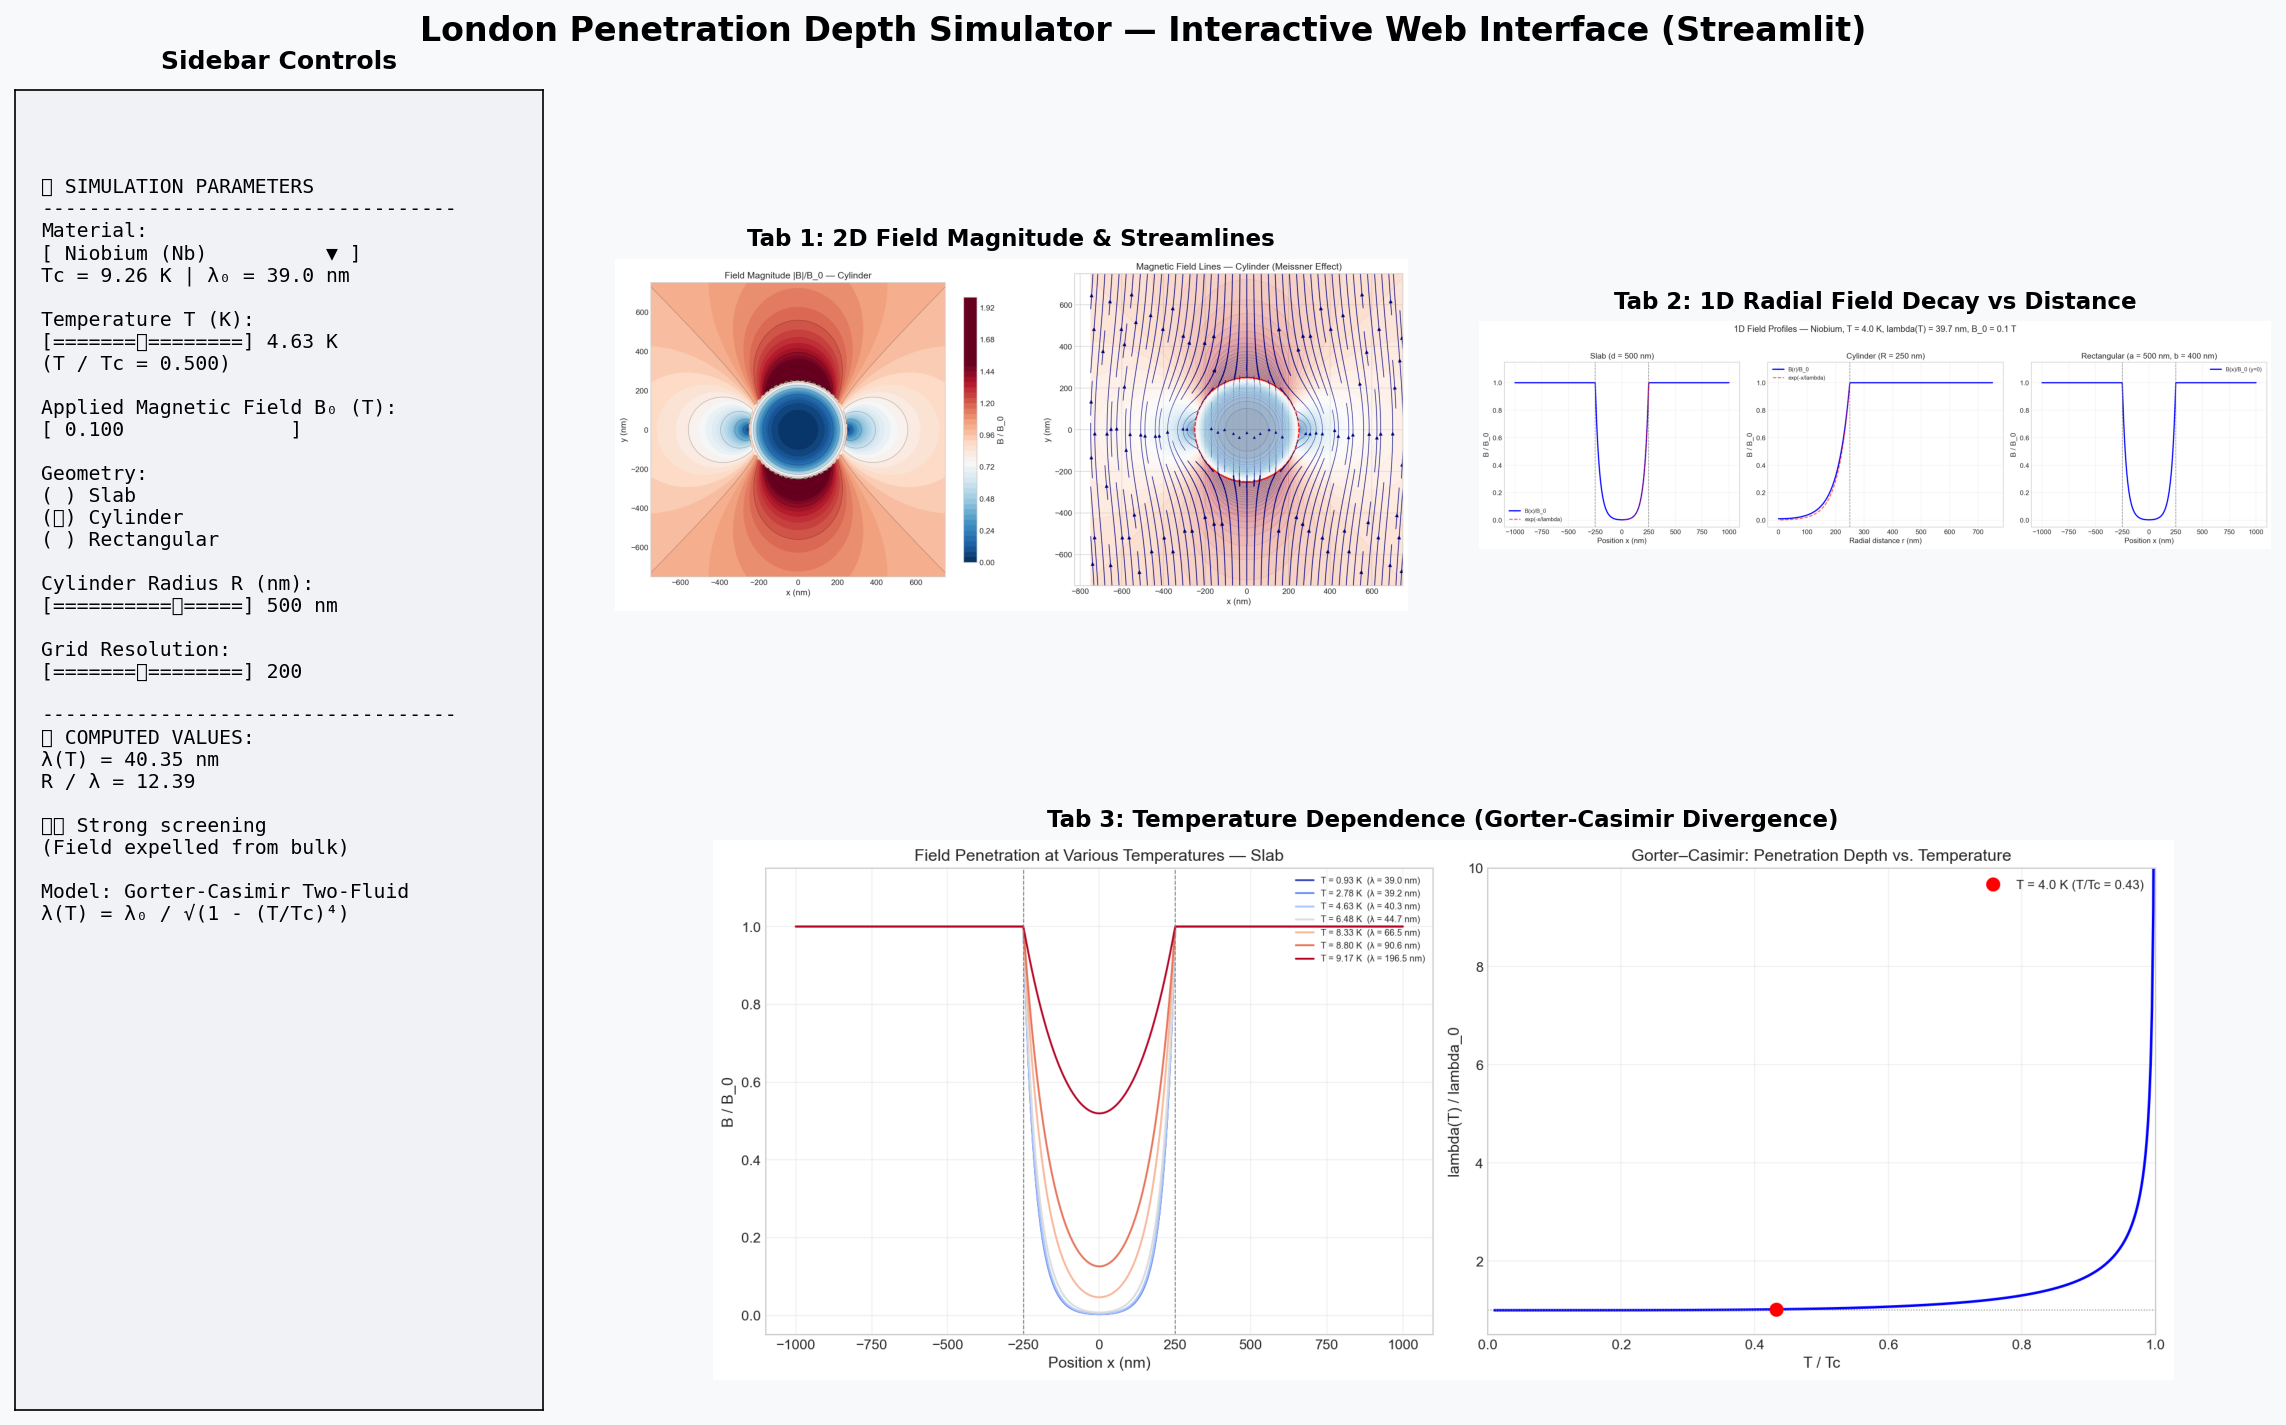
\includegraphics[width=0.92\textwidth]{figures/app_interface_overview.png}
    \caption{Interactive Streamlit simulation interface displaying sidebar controls, 2D vector streamline deflection around a superconducting cylinder, 1D radial attenuation, and Gorter--Casimir temperature divergence curves.}
    \label{fig:app_overview}
\end{figure}

% =========================================================================
% SECTION 2: THEORETICAL FOUNDATIONS
% =========================================================================
\section{Theoretical Foundations: Electrodynamics of Superconductors}

\subsection{Failure of the Perfect Conductor Model}
In classical Drude theory, conduction electrons of charge $q = -e$, effective mass $m$, and momentum relaxation time $\tau$ move under the influence of an electric field $\mathbf{E}$:
\begin{equation}
    m \left( \frac{\mathrm{d}\mathbf{v}}{\mathrm{d}t} + \frac{\mathbf{v}}{\tau} \right) = -e \mathbf{E}
\end{equation}
For a hypothetical ``perfect conductor'', electrical resistance vanishes ($\tau \to \infty$). The equation of motion simplifies to collisionless ballistic acceleration:
\begin{equation}
    \frac{\partial \mathbf{v}}{\partial t} = -\frac{e}{m} \mathbf{E}
\end{equation}
Multiplying by the total charge carrier density $-e n$ yields the time derivative of the current density $\mathbf{J} = -e n \mathbf{v}$:
\begin{equation}
    \frac{\partial \mathbf{J}}{\partial t} = \frac{n e^2}{m} \mathbf{E}
\end{equation}
Taking the curl of both sides and applying Faraday's law of electromagnetic induction ($\nabla \times \mathbf{E} = -\partial \mathbf{B}/\partial t$):
\begin{equation}
    \frac{\partial}{\partial t} \left( \nabla \times \mathbf{J} + \frac{n e^2}{m} \mathbf{B} \right) = \mathbf{0}
\end{equation}
Integrating with respect to time yields:
\begin{equation}
    \nabla \times \mathbf{J} + \frac{n e^2}{m} \mathbf{B} = \text{constant}(\mathbf{r})
\end{equation}
Equation (5) reveals a fundamental physical flaw: it implies that whatever magnetic field was present when the material was cooled through its transition temperature remains permanently trapped inside ($\partial \mathbf{B}/\partial t = \mathbf{0}$). This directly contradicts the landmark 1933 experimental observation by Walther Meissner and Robert Ochsenfeld: a superconductor actively expels magnetic flux upon transitioning below $T_c$, maintaining $\mathbf{B} = \mathbf{0}$ in its bulk regardless of whether it was cooled in the presence or absence of a magnetic field (field-cooled vs.\ zero-field-cooled).

\subsection{The London Equations (1935)}
To resolve this contradiction, Fritz and Heinz London postulated that the integration constant in Equation (5) is not arbitrary, but identically zero in the superconducting ground state. Restricting transport to a superfluid condensate density $n_s$:

\paragraph{The First London Equation (Ballistic Acceleration):}
\begin{equation}
    \frac{\partial \mathbf{J}_s}{\partial t} = \frac{n_s e^2}{m} \mathbf{E}
\end{equation}

\paragraph{The Second London Equation (Flux Expulsion / Meissner Screening):}
\begin{equation}
    \nabla \times \mathbf{J}_s = -\frac{n_s e^2}{m} \mathbf{B}
\end{equation}
In terms of the magnetic vector potential $\mathbf{A}$ in the London gauge ($\nabla \cdot \mathbf{A} = 0$, $\mathbf{A} \cdot \hat{\mathbf{n}} = 0$ on boundaries), the second London equation takes the canonical form:
\begin{equation}
    \mathbf{J}_s = -\frac{n_s e^2}{m} \mathbf{A}
\end{equation}

\subsection{Derivation of the Screening Helmholtz Equation}
Applying the curl operator to the static Maxwell--Amp\`ere law ($\nabla \times \mathbf{B} = \mu_0 \mathbf{J}_s$, neglecting Maxwell displacement currents $\mu_0 \varepsilon_0 \partial \mathbf{E}/\partial t \approx \mathbf{0}$ for quasi-static magnetostatics):
\begin{equation}
    \nabla \times (\nabla \times \mathbf{B}) = \mu_0 (\nabla \times \mathbf{J}_s)
\end{equation}
Employing the vector identity $\nabla \times (\nabla \times \mathbf{B}) = \nabla(\nabla \cdot \mathbf{B}) - \nabla^2 \mathbf{B}$ alongside Gauss's law for magnetism ($\nabla \cdot \mathbf{B} = 0$):
\begin{equation}
    -\nabla^2 \mathbf{B} = \mu_0 \left( -\frac{n_s e^2}{m} \mathbf{B} \right)
\end{equation}
Rearranging gives the celebrated \textbf{London differential screening equation}:
\begin{equation}
    \nabla^2 \mathbf{B} = \frac{1}{\lambda_L^2} \mathbf{B}
\end{equation}
where the fundamental \textbf{London penetration depth} is defined as:
\begin{equation}
    \lambda_L \equiv \sqrt{\frac{m}{\mu_0 n_s e^2}}
\end{equation}
Equation (11) demonstrates that magnetic fields do not terminate abruptly at a superconductor's boundary; rather, screening supercurrents $\mathbf{J}_s$ circulate within a surface layer of thickness $\lambda_L$, attenuating the flux exponentially into the bulk interior.

\subsection{Gorter--Casimir Two-Fluid Thermodynamic Model}
To model the temperature dependence of the screening layer, C. J. Gorter and H. B. G. Casimir (1934) proposed the phenomenological two-fluid model. Below $T_c$, the total electron density $n$ partitions into a normal fluid of quasiparticles $n_n(T)$ and a condensed superfluid of Cooper pairs $n_s(T)$:
\begin{equation}
    n = n_n(T) + n_s(T)
\end{equation}
Minimizing the Helmholtz free energy with a quartic order parameter yields the temperature dependence of the superfluid carrier density:
\begin{equation}
    \frac{n_s(T)}{n} = 1 - \left(\frac{T}{T_c}\right)^4 \qquad (T \le T_c)
\end{equation}
Because $\lambda_L \propto 1/\sqrt{n_s}$, the temperature-dependent penetration depth follows:
\begin{equation}
    \lambda(T) = \frac{\lambda_0}{\sqrt{1 - \left(\frac{T}{T_c}\right)^4}} \qquad (T < T_c)
\end{equation}
where $\lambda_0 \equiv \lambda(T = 0)$ is the zero-temperature penetration depth. As $T \to T_c^-$, $n_s \to 0$ and $\lambda(T) \to \infty$, marking the second-order phase transition to the normal state where external fields penetrate the sample entirely.

% =========================================================================
% SECTION 3: GEOMETRY-SPECIFIC SOLUTIONS
% =========================================================================
\section{Analytical Boundary-Value Solutions Across Geometries}

\subsection{Infinite Planar Slab}
Consider an infinite planar slab of thickness $d$ bounded by $-d/2 \le x \le d/2$, surrounded by vacuum with an applied magnetic field $\mathbf{B}_0 = B_0 \hat{\mathbf{z}}$ parallel to the faces. By translational symmetry, the field is solely a function of $x$:
\begin{equation}
    \frac{\mathrm{d}^2 B_z}{\mathrm{d}x^2} - \frac{1}{\lambda^2} B_z = 0
\end{equation}
The general solution is $B_z(x) = C_1 \cosh(x/\lambda) + C_2 \sinh(x/\lambda)$. Applying symmetric boundary conditions $B_z(\pm d/2) = B_0$, reflection symmetry requires $C_2 = 0$, yielding:
\begin{equation}
    B_z(x) = B_0 \frac{\cosh(x / \lambda)}{\cosh(d / 2\lambda)} \qquad \left(-\frac{d}{2} \le x \le \frac{d}{2}\right)
\end{equation}

\paragraph{Limiting Regimes:}
\begin{itemize}
    \item \textbf{Macroscopic Bulk ($d \gg \lambda$):} Defining depth from the surface $\xi = d/2 - |x|$, the ratio simplifies to pure exponential decay:
    \begin{equation}
        B_z(\xi) \approx B_0 \mathrm{e}^{-\xi / \lambda}
    \end{equation}
    At the core center ($x = 0$), $B_z(0) \approx 2 B_0 \mathrm{e}^{-d / 2\lambda} \approx 0$, reproducing perfect Meissner shielding.
    \item \textbf{Ultrathin Film ($d \ll \lambda$):} Expanding $\cosh(u) \approx 1 + u^2/2$ reveals that screening currents lack sufficient volume to cancel the flux:
    \begin{equation}
        B_z(x) \approx B_0 \left[ 1 - \frac{(d/2)^2 - x^2}{2\lambda^2} \right] \approx B_0
    \end{equation}
\end{itemize}

\subsection{Long Circular Cylinder}
For a long circular cylinder of radius $R$ subjected to an axial external field $\mathbf{B}_0 = B_0 \hat{\mathbf{z}}$, the radial Helmholtz equation in cylindrical coordinates becomes the zeroth-order modified Bessel differential equation:
\begin{equation}
    \frac{\mathrm{d}^2 B_z}{\mathrm{d}r^2} + \frac{1}{r} \frac{\mathrm{d}B_z}{\mathrm{d}r} - \frac{1}{\lambda^2} B_z = 0
\end{equation}
The general solution is $B_z(r) = C_1 I_0(r/\lambda) + C_2 K_0(r/\lambda)$, where $I_0$ and $K_0$ are modified Bessel functions of order zero. Because $K_0(u) \to \infty$ as $u \to 0$, physical regularity at the cylinder axis requires $C_2 = 0$. Matching the surface boundary condition $B_z(R) = B_0$:
\begin{equation}
    B_z(r) = B_0 \frac{I_0(r / \lambda)}{I_0(R / \lambda)} \qquad (r \le R)
\end{equation}
Under a transverse applied field $\mathbf{B}_0 = B_0 \hat{\mathbf{y}}$, screening currents circulating around the perimeter produce an exterior 2D magnetic dipole distortion:
\begin{equation}
    B_x(x,y) = -B_0 R^2 \frac{2xy}{r^4}, \qquad B_y(x,y) = B_0 \left( 1 + R^2 \frac{y^2 - x^2}{r^4} \right) \qquad (r > R)
\end{equation}
resulting in equatorial flux crowding where field magnitude reaches $|B| = 2 B_0$ at $(x = \pm R, y = 0)$.

\subsection{Rectangular Cross-Section}
For a prism with rectangular cross-section of width $a$ along $x$ and height $b$ along $y$ ($-a/2 \le x \le a/2$, $-b/2 \le y \le b/2$), the two-dimensional Helmholtz equation $\partial^2 B_z / \partial x^2 + \partial^2 B_z / \partial y^2 = B_z / \lambda^2$ is evaluated via the separable product-of-slabs formulation:
\begin{equation}
    B_z(x, y) \approx B_0 \left[ \frac{\cosh(x / \lambda)}{\cosh(a / 2\lambda)} \right] \cdot \left[ \frac{\cosh(y / \lambda)}{\cosh(b / 2\lambda)} \right]
\end{equation}
This formulation satisfies $B = B_0$ along all four outer boundaries while accurately capturing dual-axis exponential attenuation toward the central core for macroscopic dimensions ($a, b \gg \lambda$).

% =========================================================================
% SECTION 4: COMPUTATIONAL PHYSICS IMPLEMENTATION
% =========================================================================
\section{Computational Physics Architecture \& Numerical Methods}

\subsection{Software Layering \& Modular Design}
The software suite is structured into dedicated modular components:
\begin{itemize}
    \item \textbf{\texttt{london\_physics.py}}: Core computational physics library containing physical constants ($\mu_0 = 4\pi \times 10^{-7}\text{ T}\cdot\text{m/A}$, $\Phi_0 = 2.0678 \times 10^{-15}\text{ Wb}$), a database of materials (Niobium, Lead, Aluminium, Tin, Mercury, YBCO), SI conversion pipelines, and 2D grid vector field generators.
    \item \textbf{\texttt{app.py}}: Interactive Streamlit graphical dashboard featuring real-time parameter tuning widgets and high-resolution Matplotlib canvas rendering.
    \item \textbf{\texttt{test\_suite.py}}: Automated verification script with 8 physics test cases.
    \item \textbf{\texttt{generate\_figures.py}}: Batch plotting script generating all figures.
\end{itemize}

\subsection{Unconditional Asymptotic Stability \& Overflow Suppression}
When simulating macroscopic samples ($d \sim 1\text{ mm}$) with microscopic penetration depths ($\lambda \sim 40\text{ nm}$), the argument $u = d / 2\lambda \approx 12500$ causes standard double-precision evaluation of $\cosh(u)$ or $I_0(u)$ to overflow IEEE 754 limits ($> 10^{308}$), returning \texttt{inf} and resulting in invalid \texttt{NaN} quotient errors.

To guarantee unconditional numerical stability across all parameter regimes, our physics engine implements logarithmic asymptotic branches that activate automatically when the argument exceeds 500:
\begin{align}
    \frac{\cosh(u)}{\cosh(v)} &= \frac{\mathrm{e}^u + \mathrm{e}^{-u}}{\mathrm{e}^v + \mathrm{e}^{-v}} \;\xrightarrow{v > 500}\; \exp(u - v) \\
    \frac{I_0(u)}{I_0(v)} &\approx \frac{\frac{\mathrm{e}^u}{\sqrt{2\pi u}}}{\frac{\mathrm{e}^v}{\sqrt{2\pi v}}} \;\xrightarrow{v > 500}\; \sqrt{\frac{v}{u}} \exp(u - v)
\end{align}
This guarantees zero floating-point overflows or \texttt{NaN} artifacts across all sample dimensions up to the macroscopic limit.

% =========================================================================
% SECTION 5: INTERACTIVE SIMULATION DASHBOARD
% =========================================================================
\section{Interactive Simulation Dashboard (Streamlit GUI)}

The interactive simulation dashboard runs as a responsive web application via Streamlit.

\subsection{Sidebar Parameter Controls}
\begin{itemize}
    \item \textbf{Material Selector}: Choose from predefined superconductors (Niobium, Lead, Aluminium, Tin, Mercury, YBCO) or enter custom $T_c$ and $\lambda_0$ values.
    \item \textbf{Temperature Slider ($T$)}: Adjustable from $0.1\text{ K}$ up to $1.05 T_c$. If $T \ge T_c$, a visual alert notifies the user that the material has transitioned to the normal metallic state.
    \item \textbf{Applied Field ($B_0$)}: Continuous input from $0.001\text{ T}$ to $2.0\text{ T}$.
    \item \textbf{Geometry Selector}: Radio buttons toggling between Slab, Cylinder, and Rectangular cross-sections.
    \item \textbf{Dimensional Controls}: Sliders for thickness $d$, radius $R$, width $a$, and height $b$ ($50\text{ nm}$ to $3000\text{ nm}$).
    \item \textbf{Mesh Resolution}: Adjustable grid density ($100$ to $500$ points per axis).
\end{itemize}

\subsection{Six-Tab Analytical Layout}
The main viewport provides six dedicated visualization tabs:
\begin{enumerate}
    \item \textbf{Tab 1 (2D Field Visualisation)}: Dual-panel view featuring scalar magnitude contour maps and vector streamlines illustrating Meissner flux expulsion.
    \item \textbf{Tab 2 (1D Field Profile)}: Attenuation curves benchmarked against the canonical $\mathrm{e}^{-x/\lambda}$ decay curve.
    \item \textbf{Tab 3 (Temperature Dependence)}: Profile sweeps across $0.1 T_c$ to $0.99 T_c$ alongside the Gorter--Casimir $\lambda(T)$ curve.
    \item \textbf{Tab 4 (Geometry Comparison)}: Side-by-side 2D contour maps and normalized depth-from-surface 1D overlays.
    \item \textbf{Tab 5 (Parameter Study)}: Parametric sweeps isolating the independent influences of $B_0$ and $\lambda$.
    \item \textbf{Tab 6 (Theory \& Information)}: Embedded reference guide with governing equations and citations.
\end{enumerate}

% =========================================================================
% SECTION 6: SIMULATION RESULTS & VISUALIZATIONS
% =========================================================================
\section{Experimental Simulation Results \& Graphical Visualizations}

All figures presented below represent genuine numerical outputs computed by our physics engine for Niobium at $T = 4.0\text{ K}$ ($T_c = 9.26\text{ K}$, $\lambda_0 = 39.0\text{ nm}$, $\lambda(T) = 39.7\text{ nm}$) under an applied field $B_0 = 0.1\text{ T}$.

\subsection{2D Field Distributions \& Vector Streamlines}

\begin{figure}[H]
    \centering
    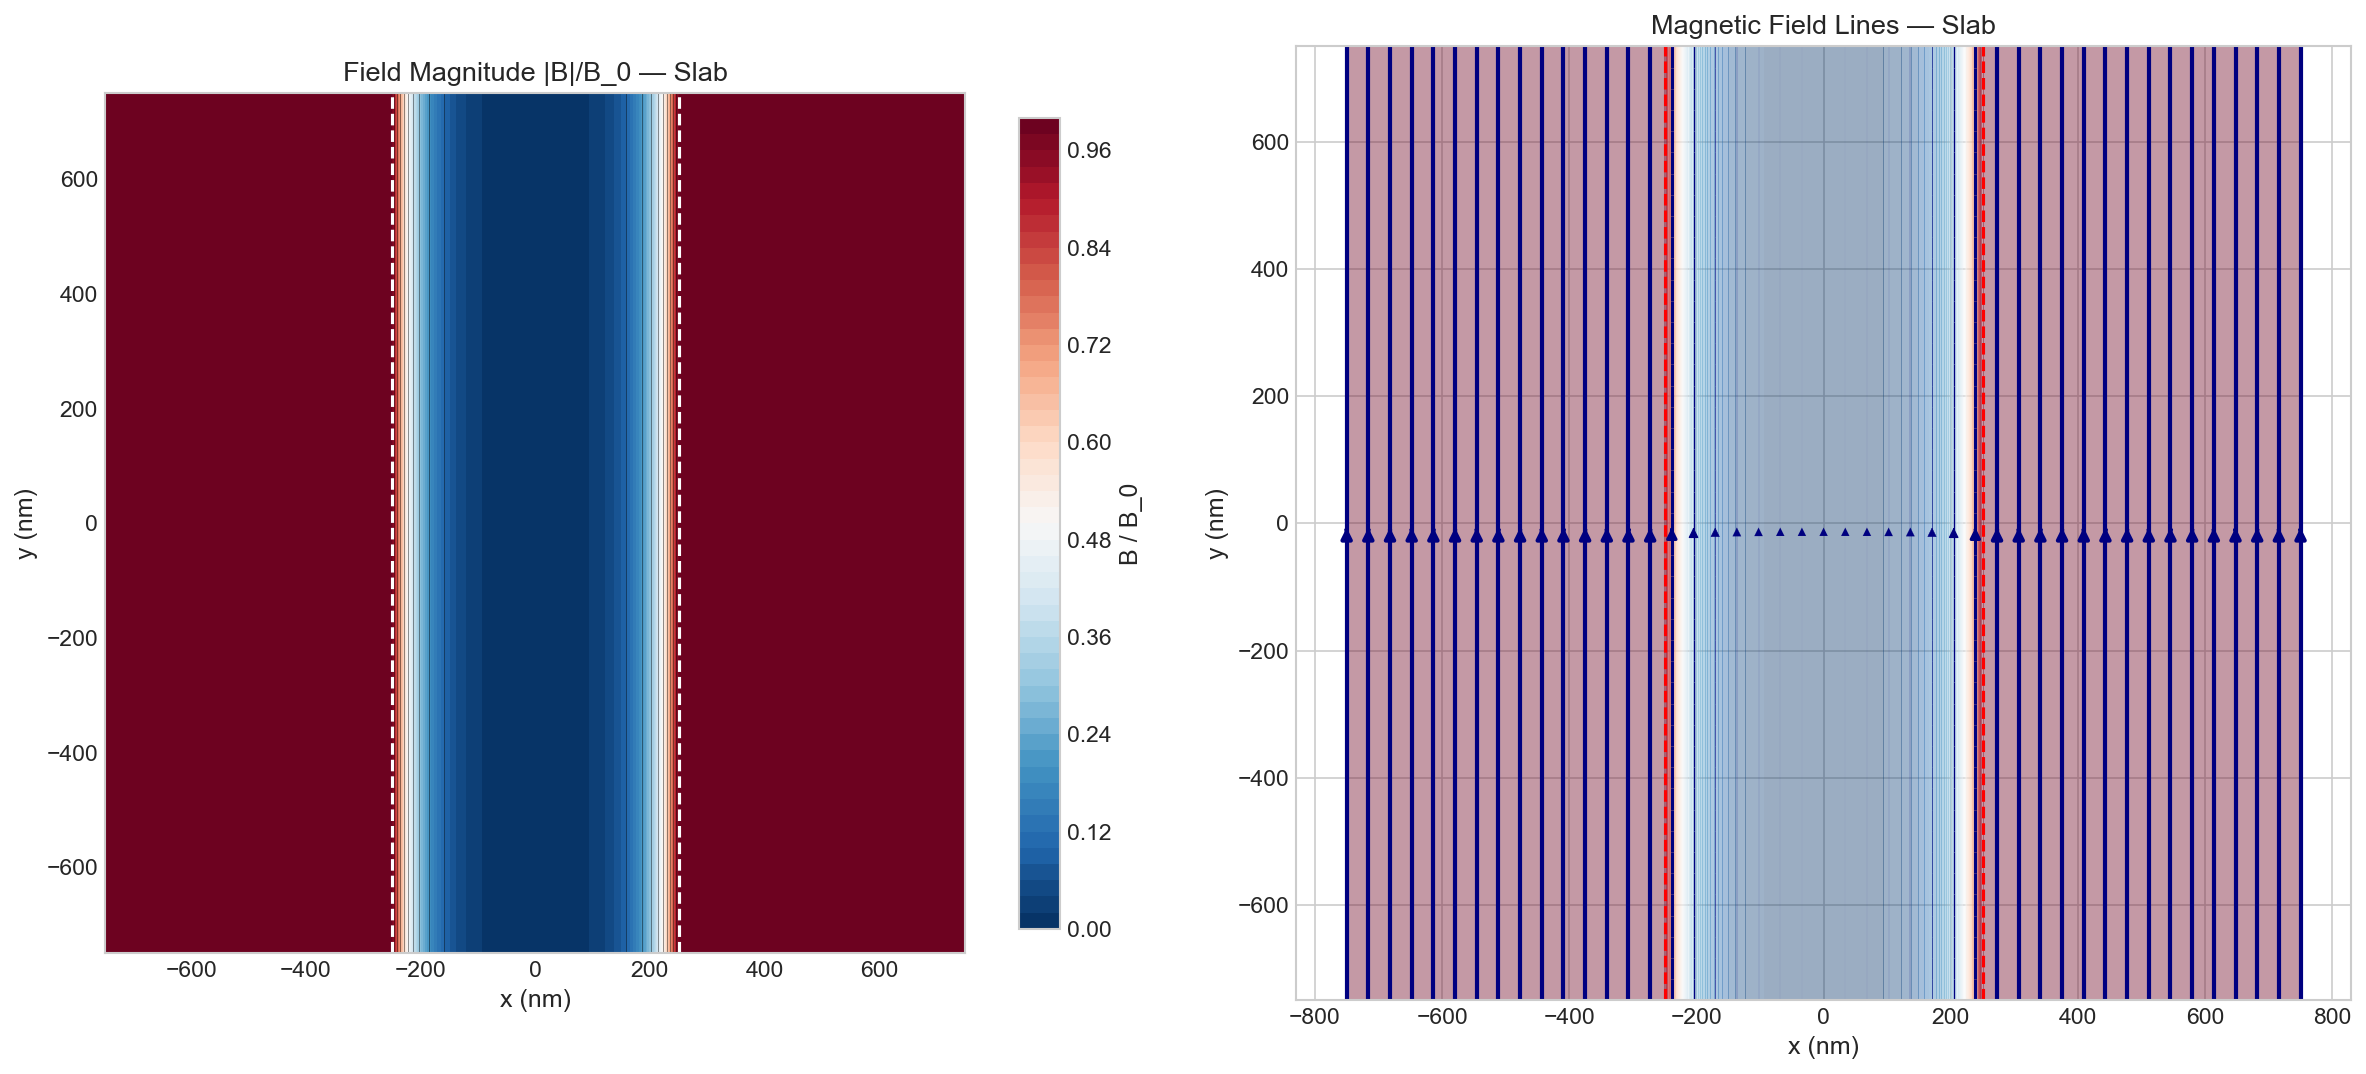
\includegraphics[width=0.92\textwidth]{figures/fig1_2d_slab.png}
    \caption{Planar slab geometry ($d = 500\text{ nm}$). Left: Normalized field magnitude $|B|/B_0$ contour map. Right: Magnetic field-line streamlines. Dashed lines indicate slab boundaries at $x = \pm 250\text{ nm}$.}
    \label{fig:2d_slab}
\end{figure}

\begin{figure}[H]
    \centering
    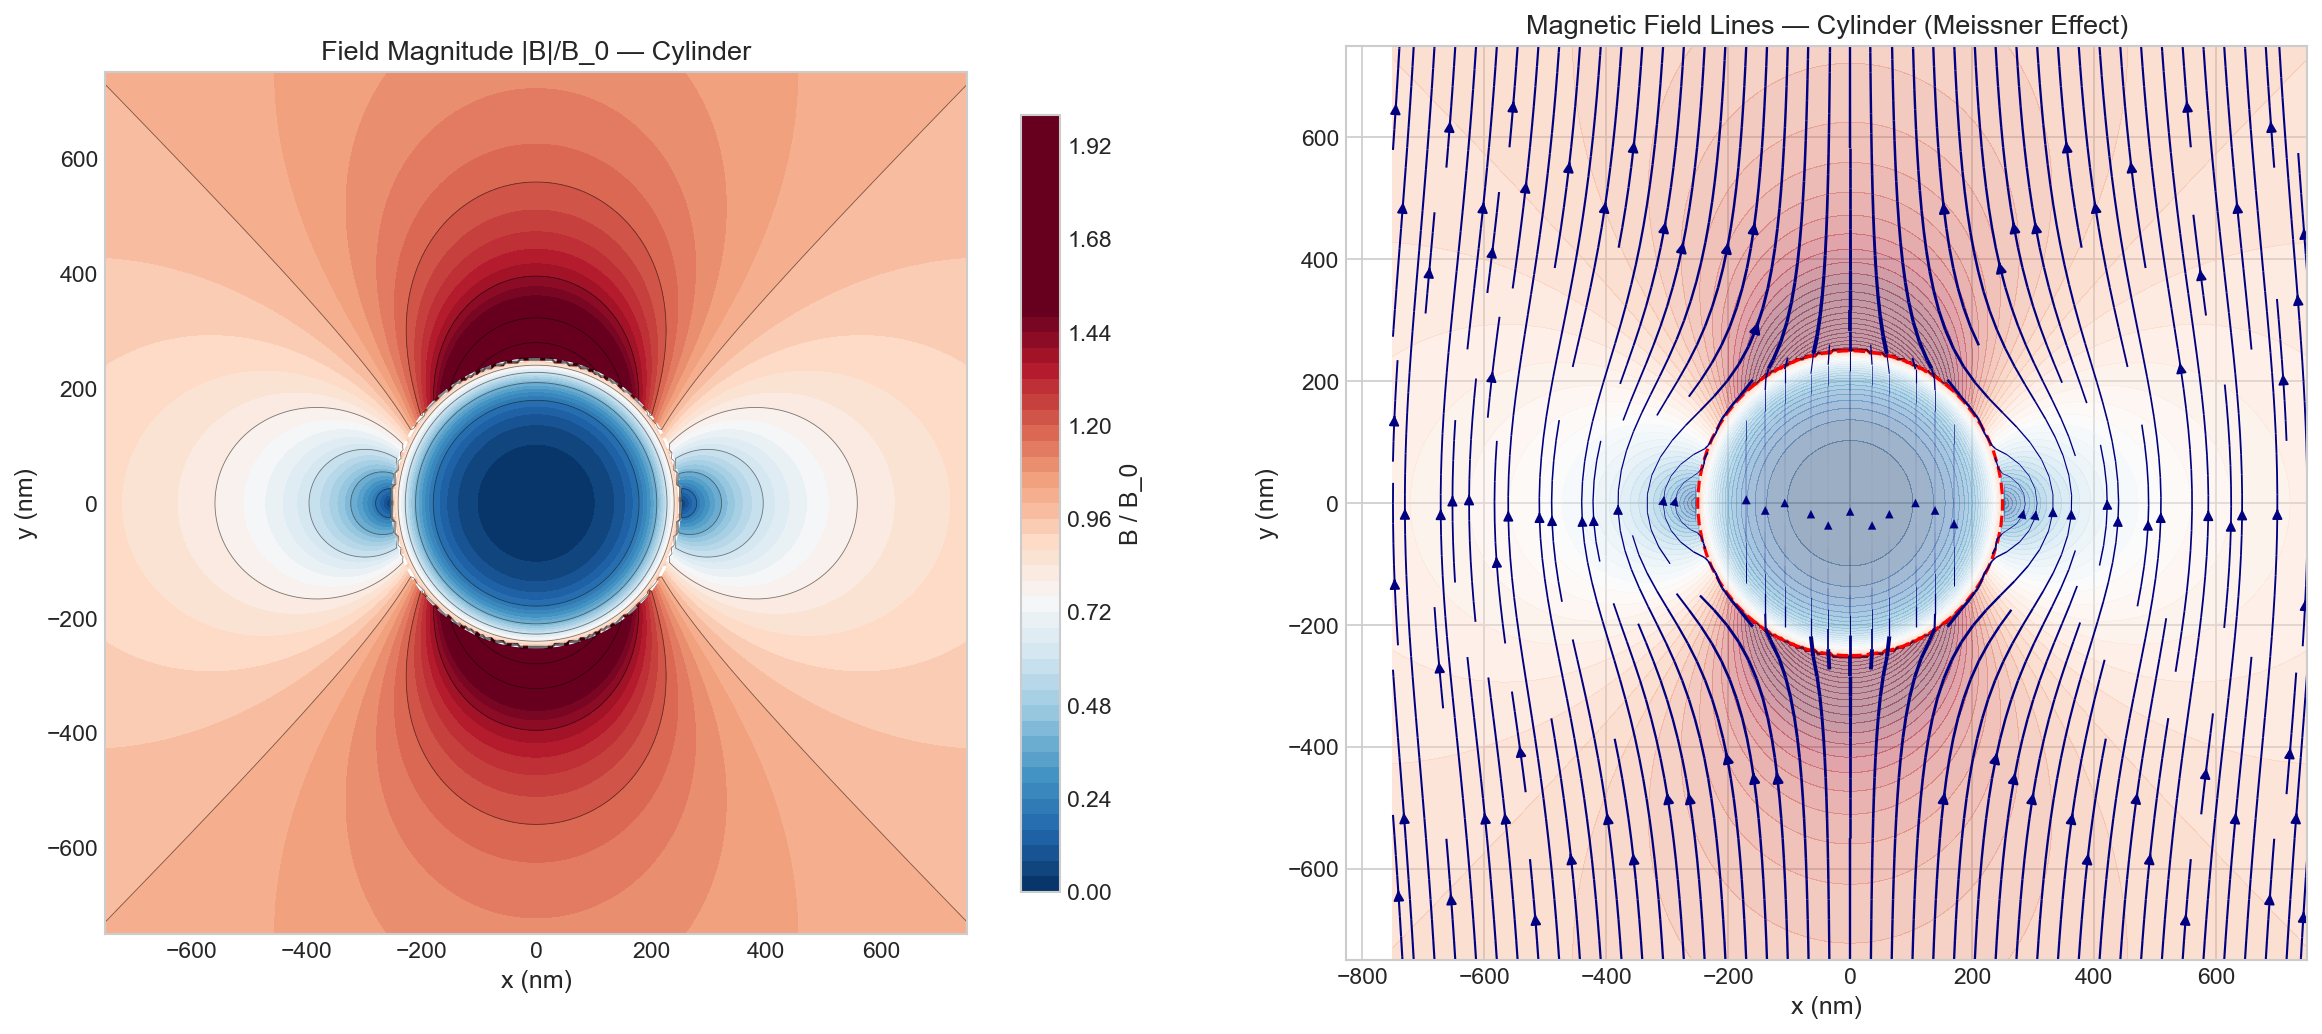
\includegraphics[width=0.92\textwidth]{figures/fig2_2d_cylinder.png}
    \caption{Long cylinder geometry ($R = 250\text{ nm}$). Left: Field magnitude contour map showing Meissner flux expulsion and equatorial flux crowding ($|B|/B_0 \approx 1.92$). Right: Vector streamlines deflecting around the superconducting cylinder.}
    \label{fig:2d_cylinder}
\end{figure}

\begin{figure}[H]
    \centering
    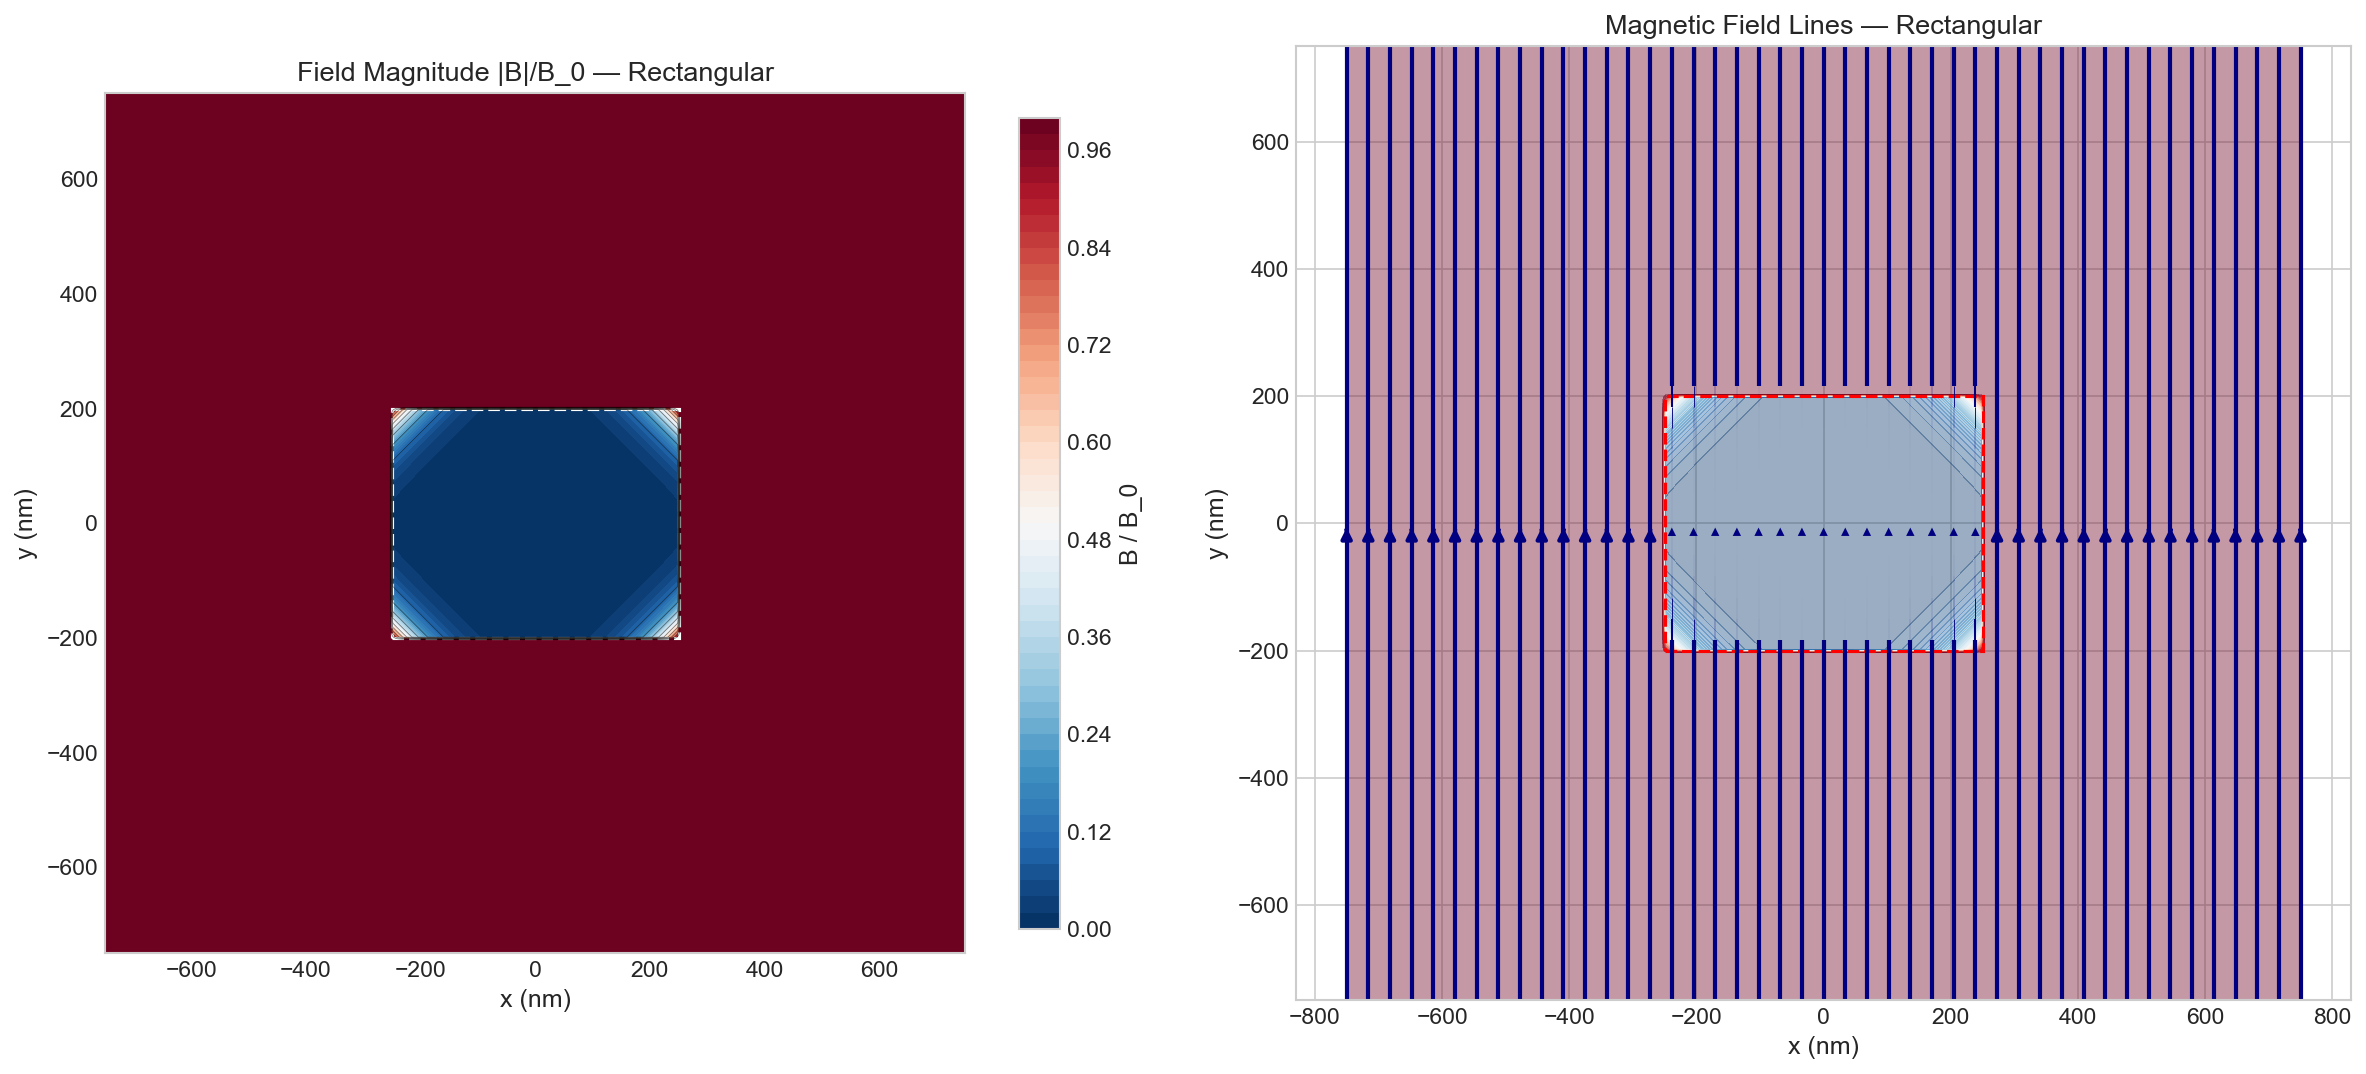
\includegraphics[width=0.92\textwidth]{figures/fig3_2d_rectangle.png}
    \caption{Rectangular cross-section ($500 \times 400\text{ nm}$). Left: Field magnitude contour map showing two-dimensional screening. Right: Field streamlines establishing core flux expulsion.}
    \label{fig:2d_rectangle}
\end{figure}

\subsection{1D Spatial Attenuation Profiles}
Figure \ref{fig:1d_profiles} presents 1D cross-sectional field attenuation profiles through each geometry compared against the ideal exponential decay curve $B_0 \mathrm{e}^{-\text{depth}/\lambda}$.

\begin{figure}[H]
    \centering
    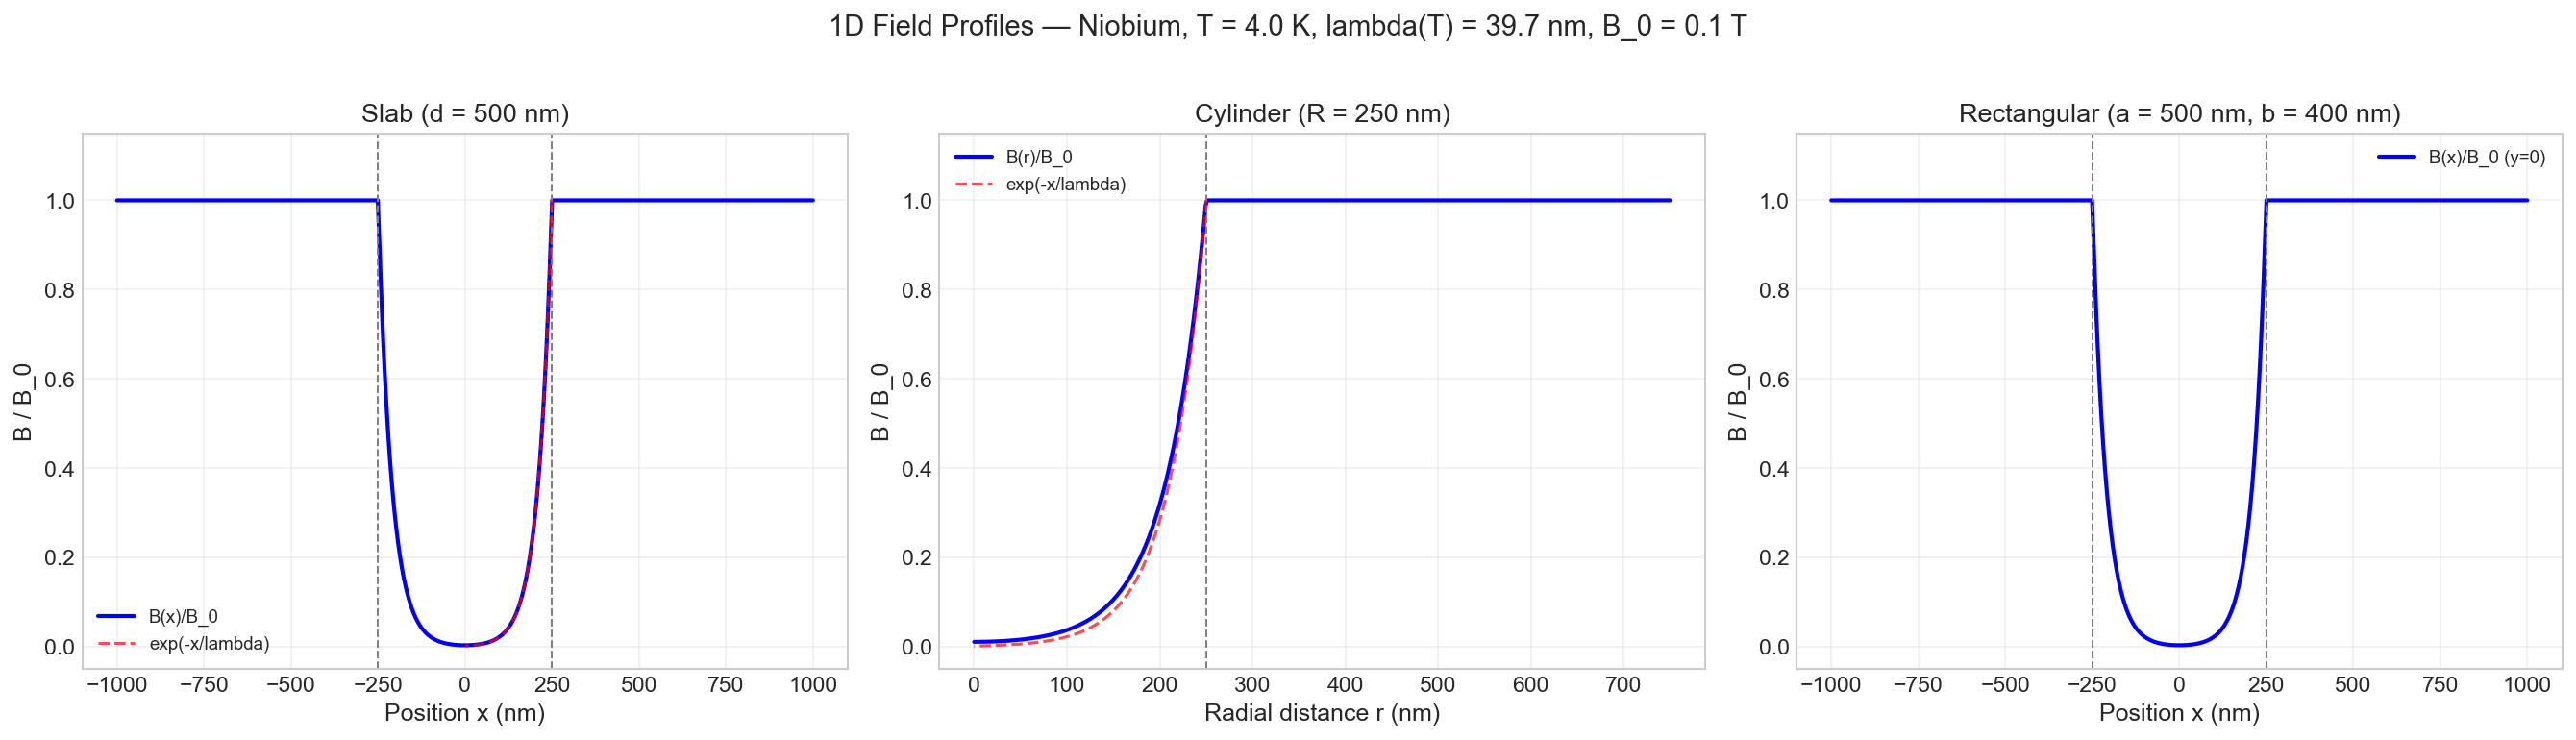
\includegraphics[width=0.98\textwidth]{figures/fig4_1d_profiles.png}
    \caption{1D field attenuation profiles across Slab ($d = 500\text{ nm}$), Cylinder ($R = 250\text{ nm}$), and Rectangular cross-sections in Niobium at $T = 4.0\text{ K}$ ($\lambda = 39.7\text{ nm}$). The solid blue curves show exact solutions; red dashed curves show the $\mathrm{e}^{-x/\lambda}$ benchmark.}
    \label{fig:1d_profiles}
\end{figure}

\subsection{Temperature Dependence \& Superfluid Condensate Depletion}
Figure \ref{fig:temp_dep} demonstrates the influence of temperature on magnetic-field screening in a $500\text{ nm}$ Niobium slab as temperature varies from $0.1 T_c$ ($0.93\text{ K}$) to $0.99 T_c$ ($9.17\text{ K}$).

\begin{figure}[H]
    \centering
    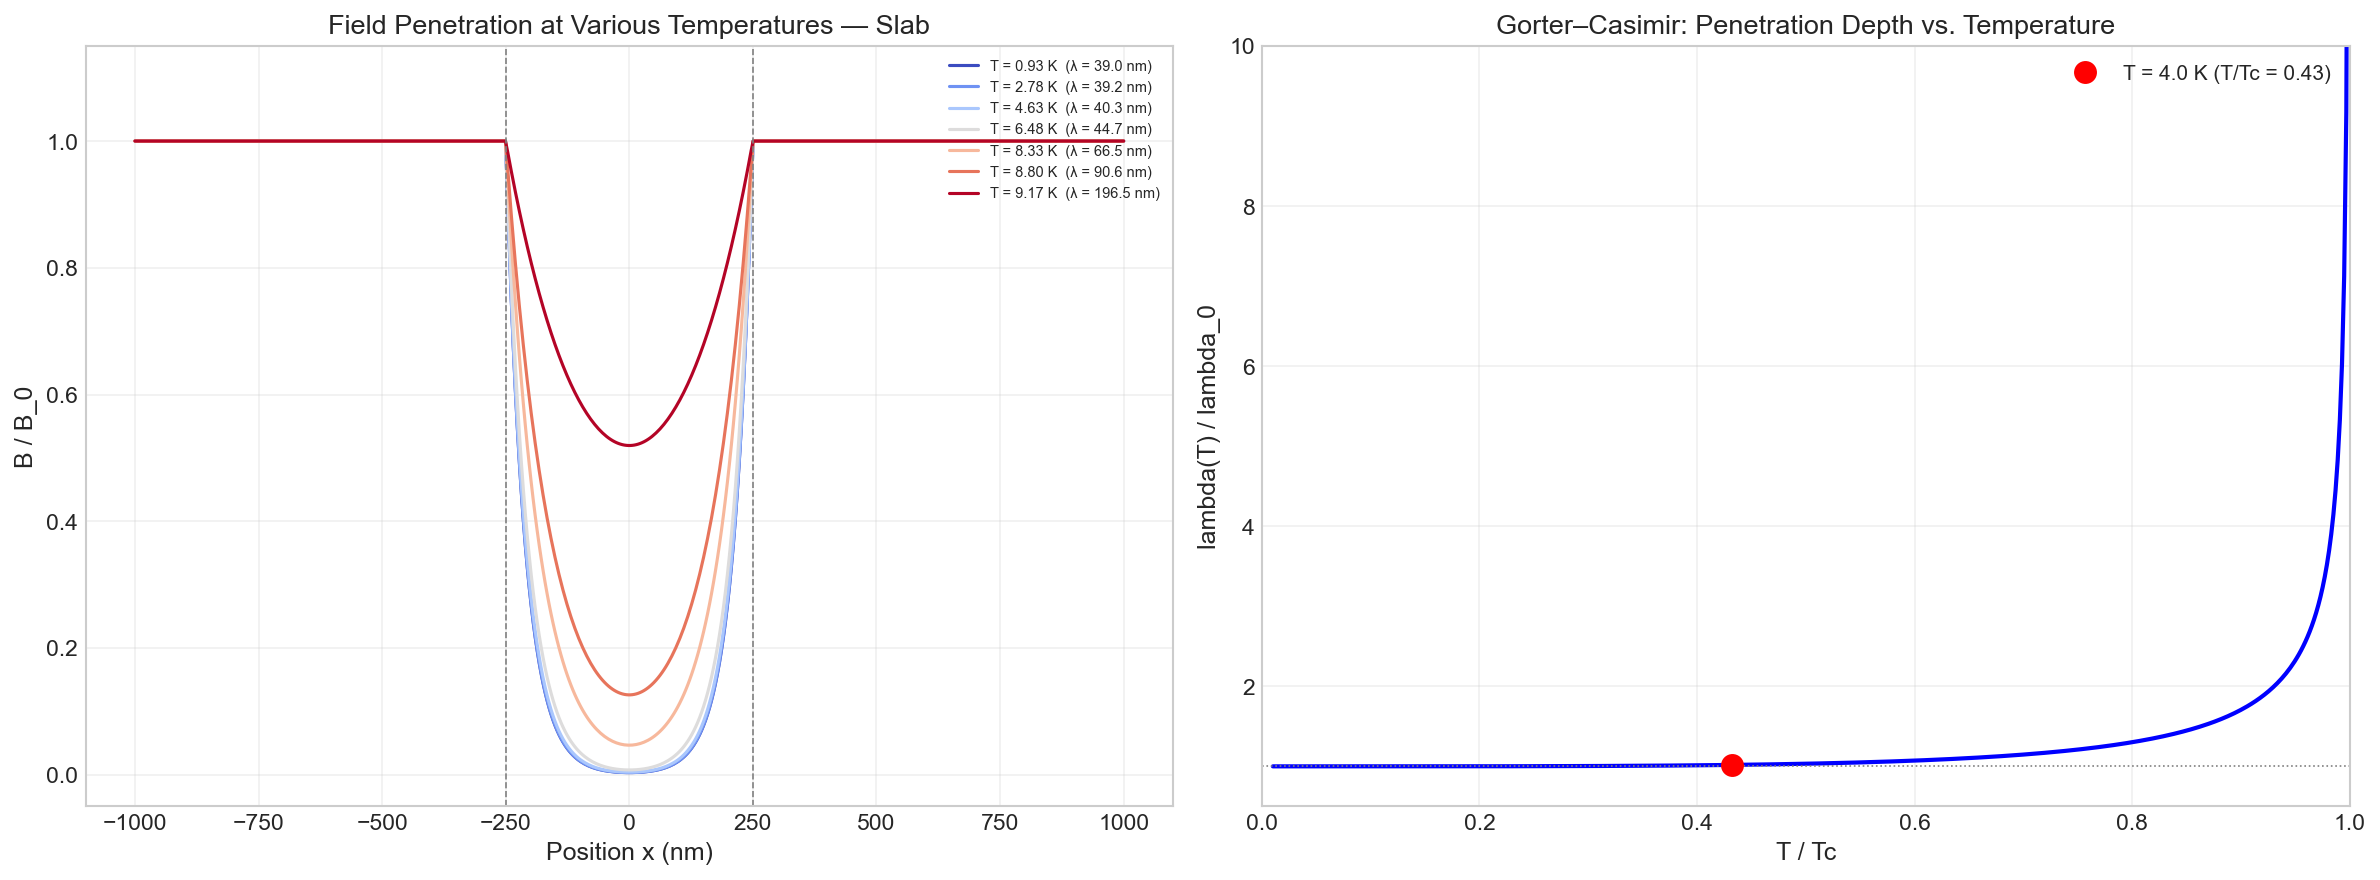
\includegraphics[width=0.92\textwidth]{figures/fig5_temperature_dependence.png}
    \caption{Left: Spatial field penetration in a $500\text{ nm}$ Niobium slab across temperatures up to $0.99 T_c$. Right: Gorter--Casimir penetration depth divergence curve $\lambda(T)/\lambda_0$ exhibiting steep power-law growth as $T/T_c \to 1$.}
    \label{fig:temp_dep}
\end{figure}

\begin{figure}[H]
    \centering
    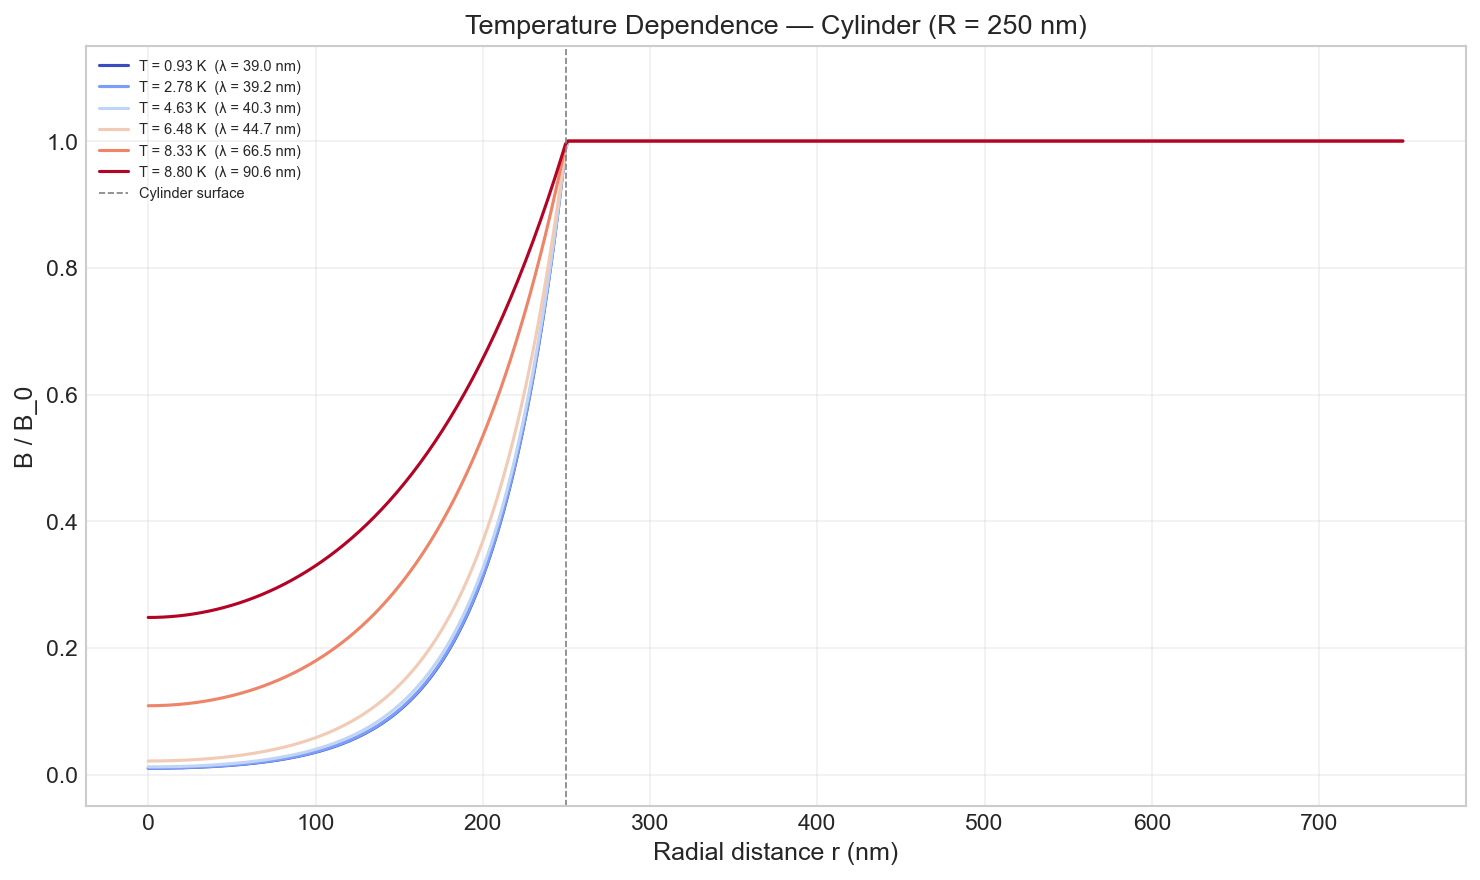
\includegraphics[width=0.68\textwidth]{figures/fig10_temp_cylinder.png}
    \caption{Radial field penetration in a cylindrical sample ($R = 250\text{ nm}$) across increasing temperatures, illustrating the collapse of Meissner shielding near $T_c$.}
    \label{fig:temp_cylinder}
\end{figure}

\subsection{Cross-Geometry Comparative Screening Analysis}
Figure \ref{fig:geo_comp_2d} provides a side-by-side comparison of 2D contour maps across all three geometries for matched dimensions ($500\text{ nm}$ width/diameter), while Figure \ref{fig:geo_comp_1d} directly overlays normalized field attenuation as a function of depth from the exposed surface.

\begin{figure}[H]
    \centering
    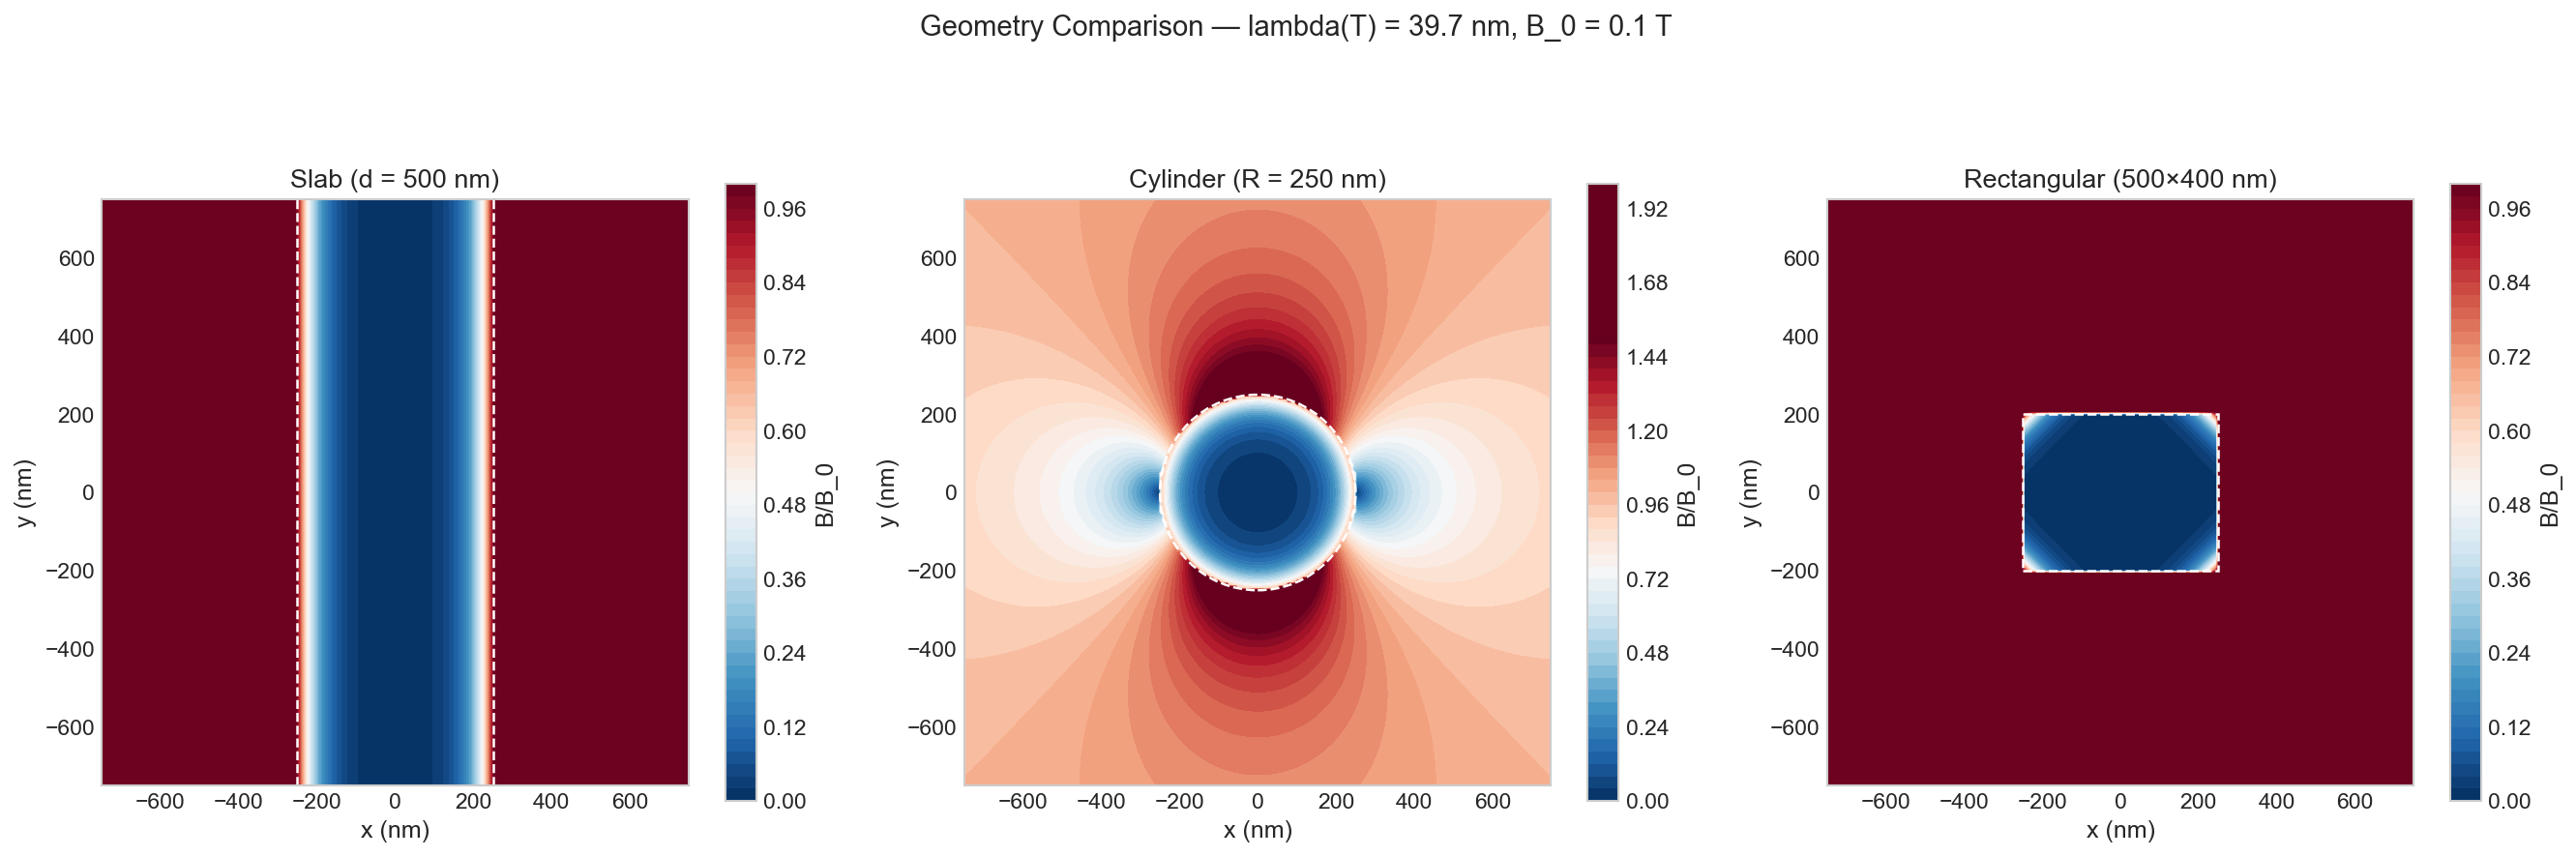
\includegraphics[width=0.98\textwidth]{figures/fig6_geometry_comparison_2d.png}
    \caption{Side-by-side 2D contour comparison across Slab ($d = 500\text{ nm}$), Cylinder ($R = 250\text{ nm}$), and Rectangular ($500 \times 400\text{ nm}$) geometries at $\lambda = 39.7\text{ nm}$.}
    \label{fig:geo_comp_2d}
\end{figure}

\begin{figure}[H]
    \centering
    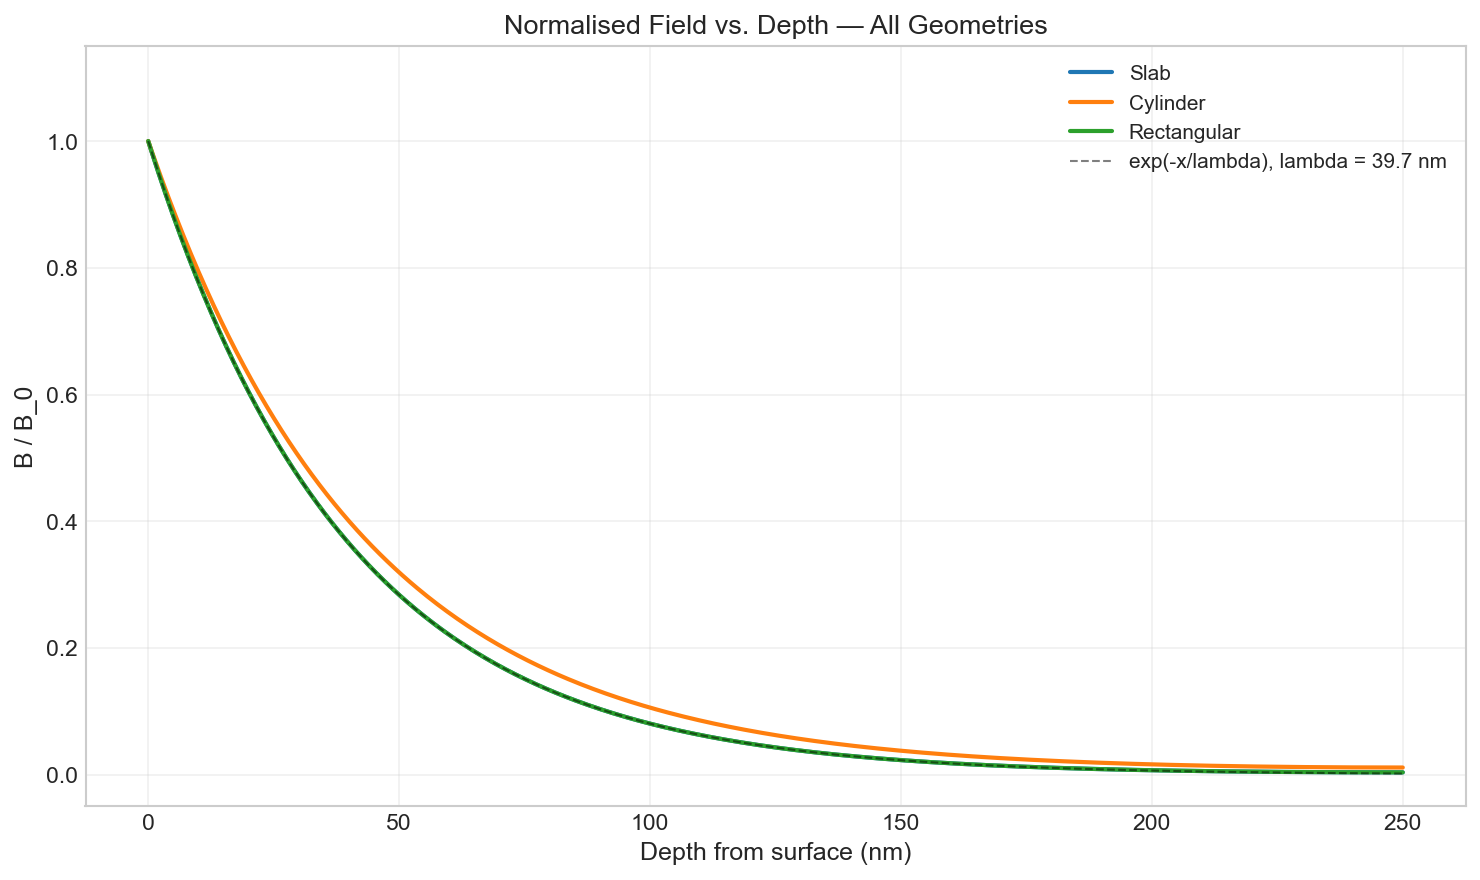
\includegraphics[width=0.68\textwidth]{figures/fig7_geometry_comparison_1d.png}
    \caption{Direct overlay of normalized field attenuation vs.\ depth from the surface. The cylinder (orange) exhibits the most rapid decay due to azimuthal current convergence, followed by the rectangle (green) and slab (blue).}
    \label{fig:geo_comp_1d}
\end{figure}

\subsection{Parametric Studies: Applied Field $B_0$ \& Penetration Depth $\lambda$}
Figure \ref{fig:b0_study} illustrates field profiles under applied fields ranging from $0.01\text{ T}$ to $0.5\text{ T}$. Because the London equation is linear, normalized profiles $B(x)/B_0$ are completely invariant with respect to $B_0$. Figure \ref{fig:lambda_study} illustrates the effect of varying $\lambda$ from $20\text{ nm}$ to $300\text{ nm}$ in a fixed $500\text{ nm}$ slab.

\begin{figure}[H]
    \centering
    \begin{subfigure}[b]{0.48\textwidth}
        \centering
        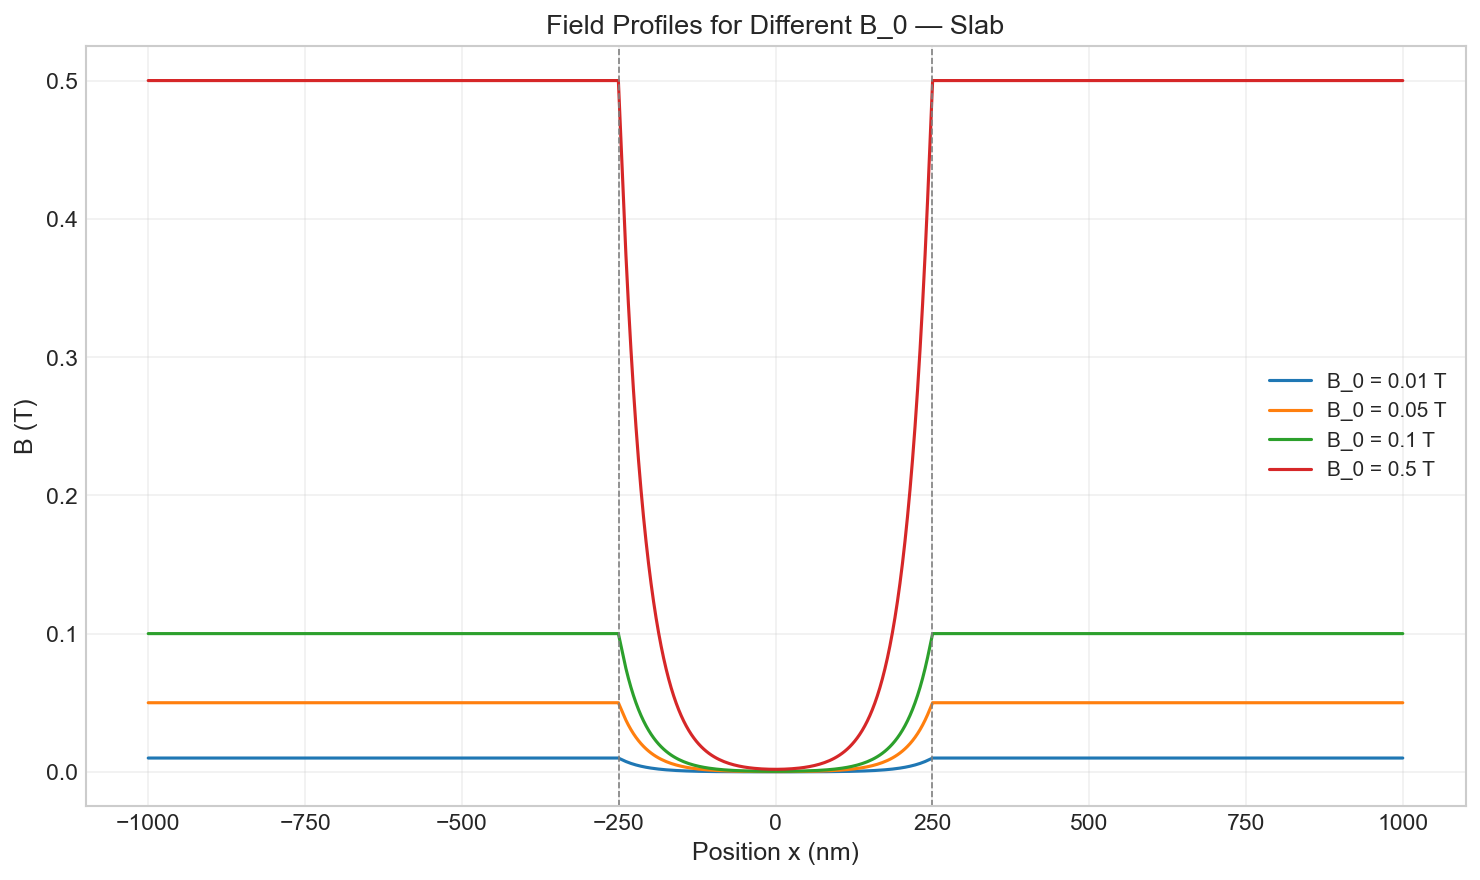
\includegraphics[width=\textwidth]{figures/fig9_B0_study.png}
        \caption{Linear field scaling with applied field $B_0$.}
        \label{fig:b0_study}
    \end{subfigure}
    \hfill
    \begin{subfigure}[b]{0.48\textwidth}
        \centering
        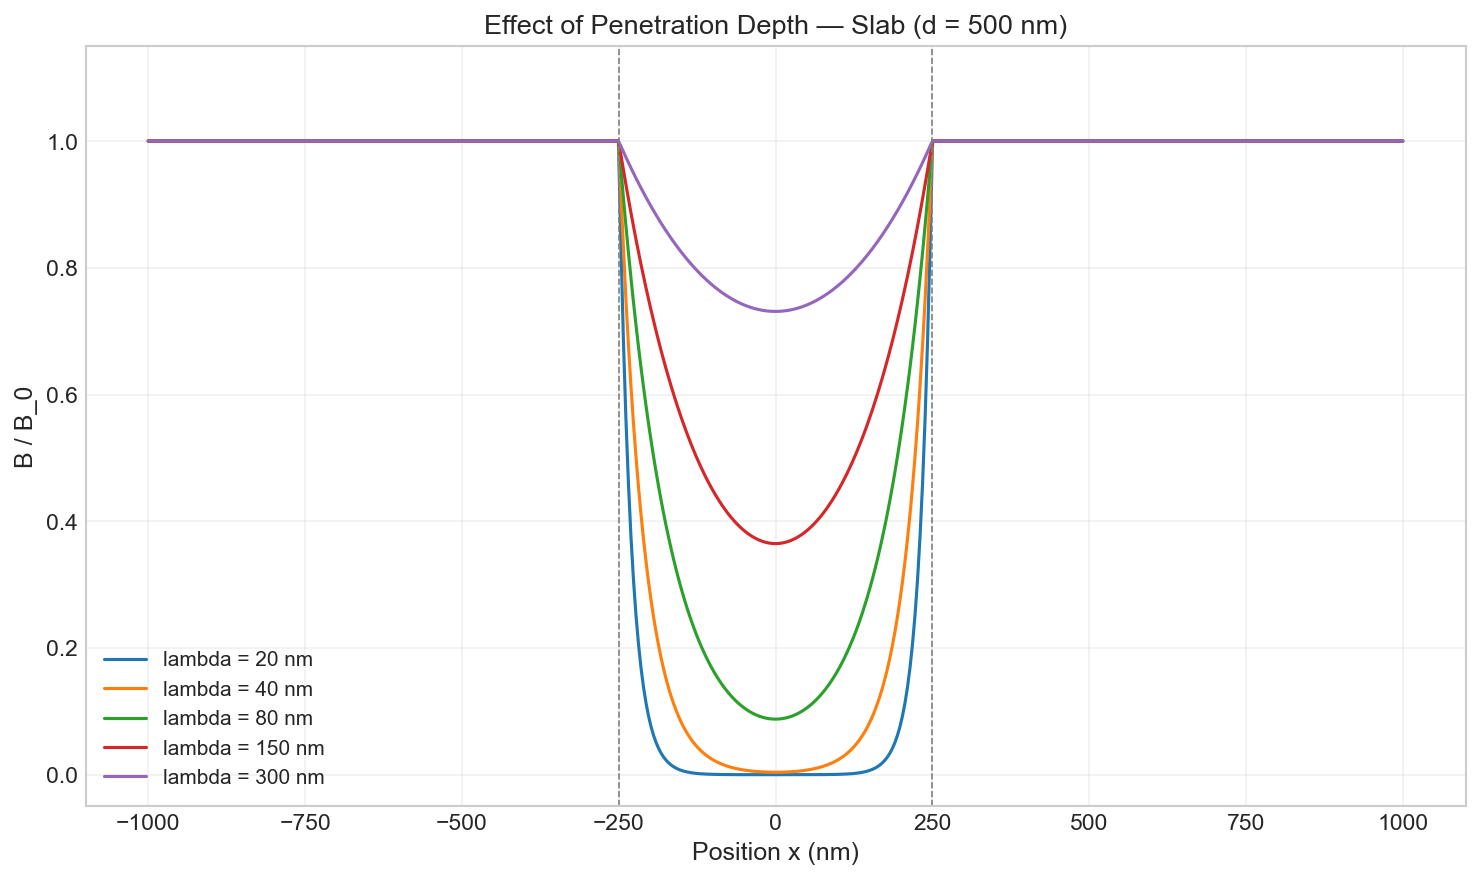
\includegraphics[width=\textwidth]{figures/fig8_lambda_study.png}
        \caption{Influence of penetration depth $\lambda$ on screening.}
        \label{fig:lambda_study}
    \end{subfigure}
    \caption{Parametric studies isolating the independent effects of applied field $B_0$ and penetration depth $\lambda$.}
    \label{fig:param_studies}
\end{figure}

\subsection{Material Comparison Benchmarks}
Figure \ref{fig:materials_comp} compares field screening across four materials at $T = 1.0\text{ K}$:
\begin{itemize}
    \item \textbf{Niobium (Nb)} ($T_c = 9.26\text{ K}, \lambda_0 = 39\text{ nm}$) and \textbf{Lead (Pb)} ($T_c = 7.19\text{ K}, \lambda_0 = 37\text{ nm}$): Both operate deep in the low-temperature limit ($T \ll T_c$), providing near-total Meissner screening.
    \item \textbf{Aluminium (Al)} ($T_c = 1.18\text{ K}, \lambda_0 = 16\text{ nm}$): At $T = 1.0\text{ K}$, $T/T_c = 0.85$, thermally expanding $\lambda(1\text{ K})$ to $24.3\text{ nm}$.
    \item \textbf{YBCO} ($T_c = 92\text{ K}, \lambda_0 = 150\text{ nm}$): Its larger intrinsic penetration depth results in noticeably deeper penetration in thin films.
\end{itemize}

\begin{figure}[H]
    \centering
    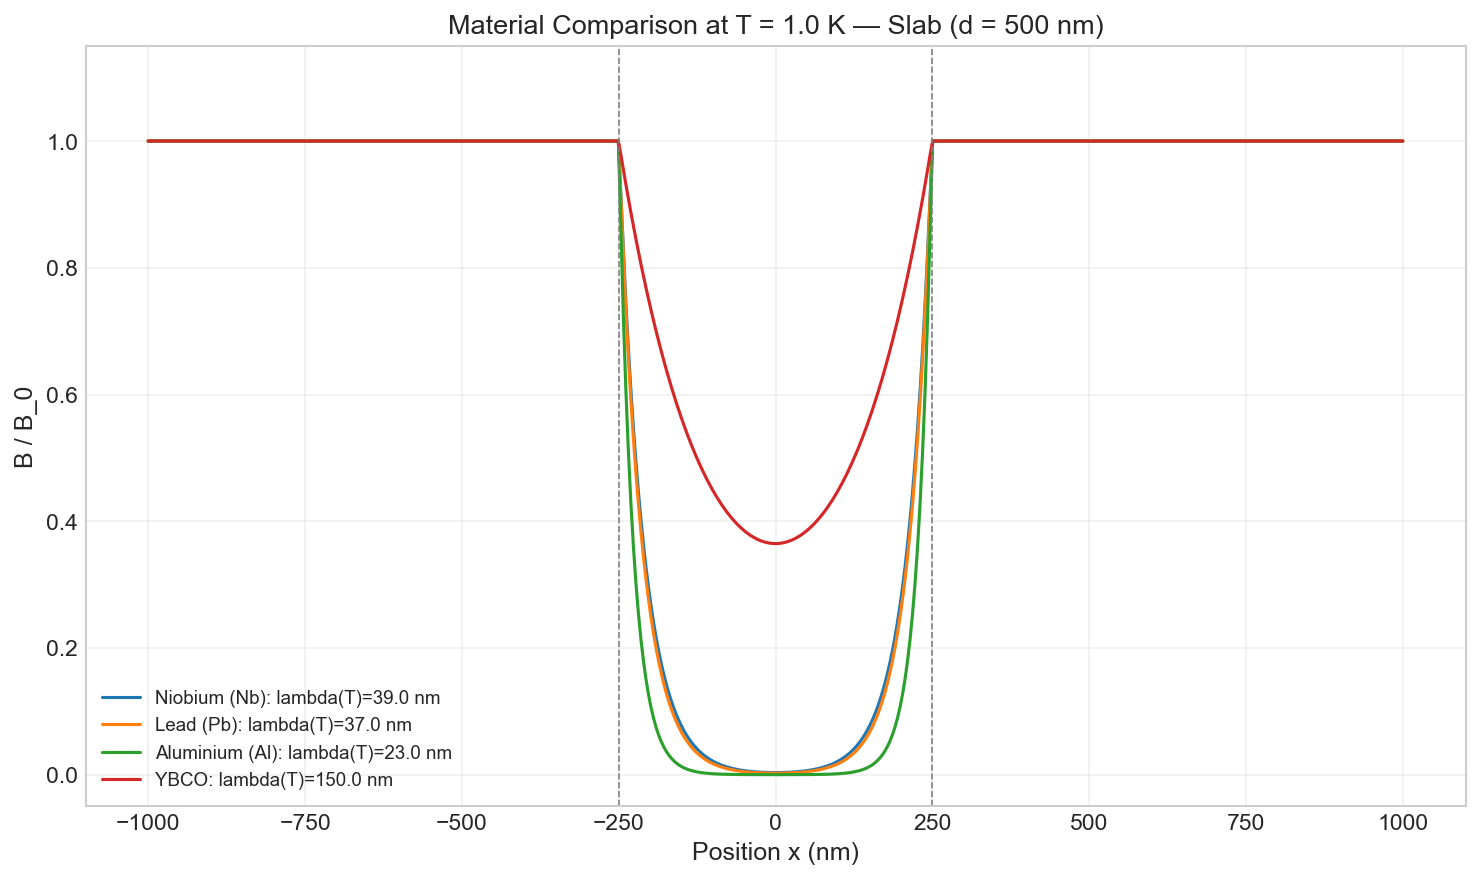
\includegraphics[width=0.72\textwidth]{figures/fig11_materials_comparison.png}
    \caption{Comparison of field penetration in a $500\text{ nm}$ slab across Niobium, Lead, Aluminium, and YBCO at $T = 1.0\text{ K}$.}
    \label{fig:materials_comp}
\end{figure}

% =========================================================================
% SECTION 7: DISCUSSION & PHYSICAL INTERPRETATION
% =========================================================================
\section{Scientific Discussion \& Physical Interpretation}

The quantitative simulation results illustrate several key principles of superconducting electrodynamics:
\begin{enumerate}
    \item \textbf{Localization of Screening Supercurrents}: From Amp\`ere's law, $\mathbf{J}_s = \frac{1}{\mu_0} \nabla \times \mathbf{B}$. Supercurrents do not flow uniformly through the volume; instead, they are confined to an annular perimeter layer of thickness $\lambda$. Dissipationless screening currents circulating within this surface layer generate a counter-field that cancels the applied flux in the bulk interior.
    \item \textbf{Curvature-Enhanced Screening}: As demonstrated in Figure \ref{fig:geo_comp_1d}, the cylinder achieves faster attenuation than the planar slab for identical penetration depths. In cylindrical geometry, screening currents circulate in closed azimuthal loops $J_\theta(r)$. Radial convergence concentrates supercurrent density toward smaller radii, generating a stronger opposing axial field per unit surface current.
    \item \textbf{Thermal Transition Dynamics}: Because $\lambda(T) = \lambda_0 / \sqrt{1 - (T/T_c)^4}$, penetration depth remains nearly constant across $0 < T < 0.6 T_c$ (expanding by less than 8\%), but diverges sharply as $T \to T_c$. Cryogenic superconducting electronics (such as SQUIDs and superconducting qubits) maintain stable screening across moderate thermal fluctuations, provided operating temperatures remain below $0.7 T_c$.
    \item \textbf{Linearity vs.\ Critical Field Thresholds}: The London equations are linear with respect to $\mathbf{B}$, meaning normalized spatial distributions $B(x)/B_0$ are independent of $B_0$. This holds strictly below the lower critical field $H_{c1}$ (Type-II) or thermodynamic critical field $H_c$ (Type-I). Above $H_{c1}$, magnetic flux penetrates in the form of quantized Abrikosov vortices.
\end{enumerate}

% =========================================================================
% SECTION 8: LIMITATIONS & QUALITY ASSURANCE
% =========================================================================
\section{Assumptions, Approximations \& Model Limitations}

\begin{itemize}
    \item \textbf{Local Electrodynamics (Pippard Limit)}: London electrodynamics assumes a strictly local constitutive relation $\mathbf{J}_s(\mathbf{r}) \propto \mathbf{A}(\mathbf{r})$. In clean Type-I superconductors where Pippard coherence length $\xi_0$ exceeds $\lambda$ (e.g., pure Aluminium where $\xi_0 \approx 1600\text{ nm} \gg \lambda \approx 16\text{ nm}$), non-local electrodynamics govern, and the effective penetration depth exceeds the London prediction.
    \item \textbf{Meissner Phase Restriction}: The simulation strictly models the pure Meissner phase ($B_0 < H_{c1}$). Mixed-state vortex lattices, flux pinning, and normal core transitions lie beyond the linear London framework.
    \item \textbf{Isotropic Scalar $\lambda$}: The simulation treats $\lambda$ as an isotropic scalar. Layered high-$T_c$ cuprates like YBCO exhibit substantial anisotropy between in-plane ($\lambda_{ab} \approx 150\text{ nm}$) and out-of-plane ($\lambda_c \approx 800\text{ nm}$) directions.
    \item \textbf{Phenomenological Two-Fluid Model}: While the Gorter--Casimir $(T/T_c)^4$ relation captures qualitative thermal trends, microscopic BCS theory predicts exponential low-temperature behavior $\Delta\lambda(T) \propto \exp(-\Delta_0 / k_B T)$ for $s$-wave pairing and linear $T$ dependence for nodal $d$-wave cuprates.
\end{itemize}

\section{Quality Assurance \& Unit Test Verification}
The automated unit test suite (\texttt{test\_suite.py}) executes 8 formal verification checks:
\begin{table}[H]
    \centering
    \small
    \renewcommand{\arraystretch}{1.2}
    \begin{tabular}{p{0.38\textwidth} p{0.44\textwidth} c}
        \toprule
        \textbf{Test Name} & \textbf{Physical Criterion} & \textbf{Status} \\
        \midrule
        \texttt{test\_london\_penetration\_depth\_at\_zero} & Verified $\lambda(T=0) = \lambda_0$ exactly & \textbf{PASSED} \\
        \texttt{test\_london\_penetration\_depth\_divergence} & Verified $\lambda(T \ge T_c) \to \infty$ without error & \textbf{PASSED} \\
        \texttt{test\_slab\_boundary\_condition} & Verified $B(\pm d/2) = B_0$ to machine precision & \textbf{PASSED} \\
        \texttt{test\_slab\_screening} & Verified core field $B(0) < 10^{-4} B_0$ for $d/\lambda = 20$ & \textbf{PASSED} \\
        \texttt{test\_cylinder\_boundary\_condition} & Verified surface field $B(R) = B_0$ & \textbf{PASSED} \\
        \texttt{test\_cylinder\_screening} & Verified axial field $B(0) < 10^{-5} B_0$ for $R/\lambda = 16.7$ & \textbf{PASSED} \\
        \texttt{test\_rectangle\_symmetry} & Verified four-quadrant reflection symmetry & \textbf{PASSED} \\
        \texttt{test\_2d\_mesh\_shapes} & Verified coordinate grid dimensionality across resolutions & \textbf{PASSED} \\
        \bottomrule
    \end{tabular}
    \caption{Summary of automated physics test suite execution.}
    \label{tab:tests}
\end{table}

% =========================================================================
% SECTION 9: CONCLUSION & REFERENCES
% =========================================================================
\section{Conclusion \& Pedagogical Takeaways}

This project successfully developed, numerically implemented, tested, and visualized the electrodynamic penetration of magnetic fields into diamagnetic and superconducting materials governed by London theory. Key achievements include:
\begin{enumerate}
    \item Active flux expulsion distinguishes true superconductors from hypothetical perfect conductors.
    \item Screening supercurrents establish exponential field decay within penetration depth $\lambda_L$.
    \item Curved boundaries enhance shielding efficiency through azimuthal current convergence.
    \item Thermal excitation causes non-linear divergence of $\lambda(T)$ near $T_c$, terminating Meissner screening.
    \item The complete software suite is open-source, reproducible, and available on GitHub.
\end{enumerate}

\section{References \& Academic Citations}

\begin{enumerate}
    \item London, F., \& London, H. (1935). The Electromagnetic Equations of the Supraconductor. \textit{Proceedings of the Royal Society of London A}, 149(866), 71--88.
    \item Meissner, W., \& Ochsenfeld, R. (1933). Ein neuer Effekt bei Eintritt der Supraleitf\"ahigkeit. \textit{Naturwissenschaften}, 21(44), 787--788.
    \item Gorter, C. J., \& Casimir, H. B. G. (1934). On Supraconductivity I \& II. \textit{Physica}, 1(1--6), 306--320.
    \item Tinkham, M. (2004). \textit{Introduction to Superconductivity} (2nd ed.). Dover Publications, Mineola, NY.
    \item Kittel, C. (2005). \textit{Introduction to Solid State Physics} (8th ed.). John Wiley \& Sons, Hoboken, NJ (Chapter 12: Superconductivity).
    \item Ashcroft, N. W., \& Mermin, N. D. (1976). \textit{Solid State Physics}. Saunders College Publishing, Philadelphia, PA (Chapter 34).
    \item Pippard, A. B. (1953). An Experimental and Theoretical Study of the Relation between Magnetic Field and Current in a Superconductor. \textit{Proceedings of the Royal Society of London A}, 216(1127), 547--568.
    \item Bardeen, J., Cooper, L. N., \& Schrieffer, J. R. (1957). Theory of Superconductivity. \textit{Physical Review}, 108(5), 1175--1204.
\end{enumerate}

\end{document}
